% !TEX program = xelatex
\documentclass[11pt,a4paper]{article}

\usepackage[italian]{babel}
\usepackage{fontspec}
\usepackage{geometry}
\geometry{margin=2.4cm}
\usepackage{amsmath,amssymb}
\usepackage{graphicx}
\usepackage{booktabs}
\usepackage{tabularx}
\usepackage{array}
\usepackage{float}
\usepackage[table,dvipsnames]{xcolor}
\usepackage{listings}
\usepackage{longtable}
\usepackage{tikz}
\usepackage{hyperref}
\usepackage{caption}
\usepackage{subcaption}

\hypersetup{
  colorlinks=true,
  linkcolor=black,
  urlcolor=blue!60!black,
  citecolor=blue!60!black
}

% Stile listings
\definecolor{codebg}{rgb}{0.97,0.97,0.97}
\definecolor{codekw}{rgb}{0.10,0.30,0.60}
\definecolor{codestr}{rgb}{0.45,0.10,0.10}
\definecolor{codecom}{rgb}{0.30,0.50,0.30}
\lstset{
  basicstyle=\ttfamily\scriptsize,
  backgroundcolor=\color{codebg},
  keywordstyle=\color{codekw}\bfseries,
  stringstyle=\color{codestr},
  commentstyle=\color{codecom}\itshape,
  language=Python,
  showstringspaces=false,
  breaklines=true,
  breakatwhitespace=true,
  numbers=left,
  numberstyle=\tiny\color{gray},
  numbersep=8pt,
  frame=single,
  framerule=0.3pt,
  rulecolor=\color{gray!50},
  tabsize=4,
  columns=fullflexible,
  keepspaces=true,
  inputencoding=utf8,
  extendedchars=true,
  literate=
    {à}{{\`a}}1 {è}{{\`e}}1 {é}{{\'e}}1 {ì}{{\`i}}1 {ò}{{\`o}}1 {ù}{{\`u}}1
    {À}{{\`A}}1 {È}{{\`E}}1 {É}{{\'E}}1 {Ì}{{\`I}}1 {Ò}{{\`O}}1 {Ù}{{\`U}}1
}

% Maschera di taglio DCT: verde = coefficiente tenuto, rosso = azzerato.
% Argomenti: #1 = F (lato blocco), #2 = d (soglia, si tiene k+ell < d).
\newcommand{\maskgrid}[2]{%
\begin{tikzpicture}[scale=0.40, every node/.style={font=\tiny}]
\pgfmathtruncatemacro{\Fm}{#1-1}
\foreach \k in {0,...,\Fm}{
  \foreach \l in {0,...,\Fm}{
    \pgfmathtruncatemacro{\s}{\k+\l}
    \ifnum\s<#2 \def\col{green!55!black} \else \def\col{red!55!black} \fi
    \fill[\col] (\l,-\k) rectangle ++(1,-1);
    \draw[white,very thin] (\l,-\k) rectangle ++(1,-1);
  }
}
\end{tikzpicture}%
}

\title{\Large \textbf{Progetto 2 -- Metodi del Calcolo Scientifico}\\[2pt]
\large Compressione di immagini in scala di grigio tramite la DCT}
\author{}
\date{Anno Accademico 2025--2026}

\begin{document}

\begin{titlepage}
\centering
\vspace*{2.5cm}
{\large Università degli Studi di Milano Bicocca\\
Scuola di Scienze\\
Dipartimento di Informatica, Sistemistica e Comunicazione}\\[0.4cm]
{\large Metodi del Calcolo Scientifico}\\[1.6cm]
{\huge\bfseries Progetto 2}\\[0.5cm]
{\Large Compressione di immagini in scala di grigio con DCT}\\[2.5cm]
\rule{10cm}{0.4pt}\\[0.6cm]
{\large\bfseries Relazione}\\[2.2cm]
\begin{tabular}{c}
Matias Bonoli\\[0.2cm]
\end{tabular}\\[2.8cm]
{\large Anno Accademico 2025--2026}\\[0.3cm]
{\large \today}
\vfill
\end{titlepage}

\tableofcontents
\vspace{1cm}
\hrule
\vspace{0.4cm}

\section{Introduzione}

Lo scopo del progetto, come descritto nella traccia, è duplice.
Nella \emph{prima parte} si chiede di implementare la Discrete Cosine
Transform bidimensionale (DCT2) in un ambiente open source e di confrontarne i
tempi di esecuzione con la versione \emph{fast} basata su FFT messa a
disposizione dalla libreria standard del linguaggio scelto.
Nella \emph{seconda parte} si chiede di realizzare un piccolo software di
compressione di immagini in scala di grigi sullo stile del JPEG (senza matrice
di quantizzazione), con la possibilità di scegliere il file, i parametri del
blocco e della soglia di taglio, e di visualizzare il risultato.

Il presente documento è la relazione formale del progetto. È organizzata come
segue: la Sezione~\ref{sec:intro} descrive linguaggio, dipendenze, convenzione di
scaling e validazione; la Sezione~\ref{sec:dct} presenta la teoria della DCT2,
l'implementazione \emph{custom} e quella \emph{fast}, la maschera di taglio e
il confronto sperimentale dei tempi; la Sezione~\ref{sec:arch} descrive
l'architettura del codice della seconda parte; la
Sezione~\ref{sec:documentazione} documenta in dettaglio le funzioni dei moduli
(inputs, outputs, comportamento); la Sezione~\ref{sec:esperimenti} raccoglie gli
esperimenti con figure, griglie e tabelle di dati; la
Sezione~\ref{sec:conclusioni} trae le conclusioni. L'Appendice~\ref{app:codice}
riporta il codice sorgente completo.

\subsection{Linguaggio e dipendenze}\label{sec:intro}

Il progetto è interamente scritto in \textbf{Python 3}. Tutti i pacchetti
utilizzati sono \emph{open source}:
\begin{itemize}
  \item \texttt{numpy}: gestione di array e operazioni vettoriali/matriciali;
  \item \texttt{scipy.fft}: contiene la DCT2 basata su FFT. Internamente
        \texttt{scipy.fft.dct} è un \emph{wrapper} di \texttt{pocketfft}, la
        stessa libreria FFT alla base di \texttt{numpy.fft};
  \item \texttt{matplotlib}: generazione di grafici e figure;
  \item \texttt{Pillow} (\texttt{PIL}): lettura e scrittura di immagini
        \texttt{.bmp};
  \item \texttt{tkinter}: interfaccia grafica, inclusa nella libreria standard
        di Python (nessuna dipendenza esterna).
\end{itemize}

La scelta di Python è motivata dal fatto che sia open-source e dal fatto che
\texttt{scipy.fft} mette a disposizione un'implementazione efficiente della DCT2
con la stessa normalizzazione richiesta dalla traccia. La
Tabella~\ref{tab:dipendenze} riassume le librerie e il loro ruolo.

\begin{table}[H]
\centering
\caption{Dipendenze del progetto e ruolo di ciascuna.}
\label{tab:dipendenze}
\begin{tabular}{lll}
\toprule
Pacchetto & Versione & Ruolo \\
\midrule
\texttt{numpy}      & $\ge 1.26$ & array, matrici, prodotti matriciali \\
\texttt{scipy.fft}  & $\ge 1.13$ & DCT/IDCT fast (pocketfft) \\
\texttt{matplotlib} & $\ge 3.8$  & grafici e figure \\
\texttt{Pillow}     & $\ge 10.0$ & lettura/scrittura \texttt{.bmp} \\
\texttt{tkinter}    & (stdlib)   & interfaccia grafica \\
\bottomrule
\end{tabular}
\end{table}

\subsection{Convenzione di scaling}\label{sec:scaling}

La traccia richiama esplicitamente l'attenzione sullo scaling della DCT, poiché
non tutte le implementazioni usano la stessa convenzione. La normalizzazione
adottata in tutto il progetto è quella della \textbf{DCT2 ortonormale}:
\[
\alpha_0 = \frac{1}{\sqrt{N}}, \qquad
\alpha_k = \sqrt{\frac{2}{N}} \quad \text{per } k>0.
\]
Con questa scelta la matrice $D$ della trasformata è \emph{ortogonale}
($D^{-1}=D^\top$), e in \texttt{scipy.fft} corrisponde all'opzione
\texttt{norm='ortho'} di \texttt{scipy.fft.dct}. Tutto il codice del progetto
adotta questa convenzione, sia per la versione \emph{custom} sia per quella
\emph{fast}.

\subsection{Validazione}\label{sec:validazione}

Per verificare lo scaling si sono riprodotti i due casi test forniti dalla
traccia: la DCT monodimensionale della prima riga del blocco $1\times 8$ e la
DCT2 del blocco $8\times 8$. La riga di riferimento
\[
231\quad 32\quad 233\quad 161\quad 24\quad 71\quad 140\quad 245
\]
deve essere trasformata, dalla DCT monodimensionale, in
\[
4.01\mathrm{e}{+}02 \quad 6.60\mathrm{e}{+}00 \quad 1.09\mathrm{e}{+}02
\quad -1.12\mathrm{e}{+}02 \quad 6.54\mathrm{e}{+}01 \quad 1.21\mathrm{e}{+}02
\quad 1.16\mathrm{e}{+}02 \quad 2.88\mathrm{e}{+}01.
\]
Il confronto numerico, implementato in \texttt{test\_assignment.py}, dà i
seguenti risultati, riassunti nella Tabella~\ref{tab:validazione}:
\begin{itemize}
  \item \emph{custom} vs \texttt{scipy.fft} (\texttt{norm='ortho'}): errore
        massimo $\sim 10^{-13}$ (precisione di macchina);
  \item \emph{custom/fast} vs tabella della traccia: errore massimo dell'ordine
        dell'unità sulla terza cifra significativa, dovuto all'arrotondamento a
        $3$ cifre sui valori di riferimento;
  \item round-trip $\mathrm{IDCT2}(\mathrm{DCT2}(A)) = A$ accurato a meno di
        $10^{-13}$, come ci si attende da una trasformazione ortogonale.
\end{itemize}

\begin{table}[H]
\centering
\caption{Esiti dei test di validazione (\texttt{test\_assignment.py}).}
\label{tab:validazione}
\begin{tabular}{lll}
\toprule
Test & Confronto & Errore massimo \\
\midrule
DCT 1D, riga $1\times 8$  & custom vs traccia      & $\sim 1$ su $3^a$ cifra \\
DCT 1D, riga $1\times 8$  & custom vs scipy.fft    & $\sim 10^{-13}$ \\
DCT 2D, blocco $8\times 8$& custom vs traccia      & $\sim 1$ su $3^a$ cifra \\
DCT 2D, blocco $8\times 8$& custom vs fast         & $\sim 10^{-13}$ \\
Round-trip IDCT2(DCT2(A)) & ricostruzione vs $A$   & $\sim 10^{-13}$ \\
Maschera $k+\ell<d$, $F=4$& confronto con atteso   & esatto (bool) \\
\bottomrule
\end{tabular}
\end{table}

\section{Discrete Cosine Transform}\label{sec:dct}

\subsection{Richiami teorici}

Partendo dalla teoria delle serie di Fourier, la DCT nasce dal desiderio di
approssimare un segnale campionato evitando il fenomeno di Gibbs. L'idea,
descritta nelle note del corso, è di \emph{riflettere} la funzione rispetto
all'asse delle ordinate in modo da renderla pari e poi periodizzarla di periodo
$2L$: in questo modo si eliminano le discontinuità artificiali che la semplice
replicazione introduceva, e tutti i coefficienti $b_k$ (associati ai seni)
sono nulli, lasciando una \emph{serie dei coseni}.

Nel caso discreto, data una funzione campionata in $N$ punti
\[
t_i = \frac{2i+1}{2N}, \qquad i=0,\dots,N-1,
\]
i vettori di base sono
\[
(w_k)_i = \cos\!\left(\frac{k\pi(2i+1)}{2N}\right), \qquad k=0,\dots,N-1.
\]
Si dimostra (osservando le identità trigonometriche di Werner) che tali
vettori sono \emph{ortogonali}, con $w_0\!\cdot\! w_0 = N$ e
$w_k\!\cdot\! w_k = N/2$ per $k>0$. Dividendo per il valore corrispondente si
ottiene una base \emph{ortonormale}. Il coefficiente $a_k$ si calcola allora
come
\[
a_k = \frac{v\cdot w_k}{w_k\cdot w_k},
\]
operazione che non coinvolge gli altri coefficienti: ogni $a_k$ è calcolabile
indipendentemente dagli altri. La procedura che costruisce i coefficienti $a_k$
è la \textbf{Discrete Cosine Transform} (DCT); quella inversa è la
\textbf{IDCT}.

Un fatto centrale per la compressione è il seguente: \emph{più la funzione è
liscia, più i coefficienti della DCT decadono rapidamente} all'aumentare di
$k$. Per una funzione con forti oscillazioni o discontinuità (come una
funzione casuale) i coefficienti non decadono e il taglio delle alte frequenze
introduce artefatti. Questo giustifica l'efficacia della DCT nella compressione
di immagini naturali, tipicamente localmente lisce.

\subsection{Estensione al caso bidimensionale e matrice di trasformazione}

La DCT si estende al caso bidimensionale sfruttando la \emph{separabilità} del
nucleo coseno. Per una matrice quadrata $f\in\mathbb{R}^{N\times N}$,
\[
c = D\, f\, D^\top,
\]
dove $D\in\mathbb{R}^{N\times N}$ è la matrice ortonormale della DCT, con
\[
D_{k,i} = \alpha_k \cos\!\left(\frac{k\pi(2i+1)}{2N}\right), \qquad
\alpha_0 = \tfrac{1}{\sqrt{N}},\ \alpha_k = \sqrt{\tfrac{2}{N}}\ (k>0).
\]
Equivalentemente si applica la DCT2 prima a tutte le colonne e poi a tutte le
righe. Essendo $D$ ortogonale, l'inversa è la trasposta:
$f = D^\top c\, D$.

\subsection{DCT2 \guillemotleft custom\guillemotright}\label{sec:custom}

L'implementazione didattica (funzione \texttt{dct\_2d\_homemade} in
\texttt{dct\_utils.py}) costruisce esplicitamente la matrice $D$ e calcola la
DCT2 come $D\, f\, D^\top$. La matrice viene assemblata con
\texttt{numpy} senza cicli espliciti sul campione spaziale:
\[
\texttt{matrix[k,:]} = \alpha_k \cos\!\left(\frac{k\pi(2i+1)}{2N}\right).
\]
Poiché ogni prodotto matrice--matrice costa $O(N^3)$ e se ne eseguono due, il
costo asintotico complessivo è $O(N^3)$.

\subsection{DCT2 della libreria (fast, FFT-based)}\label{sec:fast}

La versione \emph{fast} usa \texttt{scipy.fft.dctn} con \texttt{type=2} e
\texttt{norm='ortho'}, che corrisponde esattamente alla DCT2 ortonormale di
cui sopra. Internamente \texttt{scipy.fft} è un \emph{wrapper} di
\texttt{pocketfft}, una FFT in precisione doppia scritta in C. La DCT2 viene
calcolata via FFT su un vettore di lunghezza $2N$, con costo $O(N\log N)$ nel
caso 1D e $O(N^2\log N)$ nel caso 2D (applicata a righe e colonne).

\subsection{La maschera di taglio delle frequenze}\label{sec:maschera}

La compressione opera azzerando i coefficienti $c_{k\ell}$ con $k+\ell\ge d$,
ossia quelli a destra dell'antidiagonale individuata da $d$. Indicando con
verde i coefficienti \emph{conservati} e con rosso quelli \emph{azzerati}, la
Figura~\ref{fig:masks} mostra la maschera per diverse coppie $(F,d)$. Il caso
$F=10$, $d=7$ riproduce l'esempio della traccia.

\begin{figure}[H]
\centering
\begin{tabular}{ccc}
\maskgrid{8}{0} & \maskgrid{8}{2} & \maskgrid{8}{5} \\
$F=8,\ d=0$ & $F=8,\ d=2$ & $F=8,\ d=5$ \\[6pt]
\maskgrid{8}{8} & \maskgrid{8}{14} & \maskgrid{10}{7} \\
$F=8,\ d=8$ & $F=8,\ d=14$ & $F=10,\ d=7$ (traccia) \\
\end{tabular}
\caption{Maschere di taglio: in verde i coefficienti con $k+\ell<d$ (tenuti),
in rosso quelli con $k+\ell\ge d$ (azzerati). Per $d=0$ si azzerano tutti; per
$d=2F-2$ si conserva tutto tranne $c_{F-1,F-1}$.}
\label{fig:masks}
\end{figure}

I due valori estremi della soglia $d$ corrispondono a:
\begin{itemize}
  \item $d=0$: tutti i coefficienti del blocco vengono azzerati (l'immagine
        ricomposta è grigio uniforme, al valore medio del blocco);
  \item $d=2F-2$: si conserva ogni coefficiente tranne $c_{F-1,F-1}$ (il
        singolo coefficiente in alto a destra in frequenza).
\end{itemize}
Il numero di coefficienti conservati, e quindi la frazione di informazione
mantenuta, dipende solo da $F$ e $d$ e vale
\[
n_{\text{kept}}(F,d) = \#\{(k,\ell): k+\ell<d\} = \sum_{j=0}^{d-1}\min(j+1,F,\,2F-1-j),
\]
con $n_{\text{kept}}/F^2$ che va da $0$ (per $d=0$) a $(F^2-1)/F^2$ (per
$d=2F-2$). La Tabella~\ref{tab:kept} riporta i valori effettivi per le
configurazioni usate negli esperimenti.

\begin{table}[H]
\centering
\caption{Numero e percentuale di coefficienti conservati per blocco al
variare di $(F,d)$.}
\label{tab:kept}
\begin{tabular}{rrrrrrrrrrrr}
\toprule
$F=8$ & & \multicolumn{4}{c}{$d$} & & $F=16$ & \multicolumn{4}{c}{$d$} \\
\cmidrule{3-6}\cmidrule{8-11}
 & & 2 & 5 & 8 & 14 & & & 4 & 10 & 20 & 30 \\
\midrule
tenuti     & & 3 & 15 & 36 & 63 & & tenuti     & 10 & 55 & 191 & 256 \\
\%         & & 4.7 & 23.4 & 56.3 & 98.4 & & \% & 3.9 & 21.5 & 74.2 & 99.6 \\
\bottomrule
\end{tabular}
\end{table}

\subsection{Confronto sperimentale dei tempi}\label{sec:tempi}

Il confronto è stato eseguito su matrici quadrate casuali $N\times N$, con
$N\in\{8,16,32,64,128,256,512,768,1024\}$. Per ogni $N$ si è preso il tempo
minimo su $3$ esecuzioni, in modo da ridurre il rumore del sistema operativo.
Il grafico utilizza scala logaritmica solo sulle ordinate (semilog-$y$), come
richiesto dalla traccia.

\begin{figure}[H]
\centering
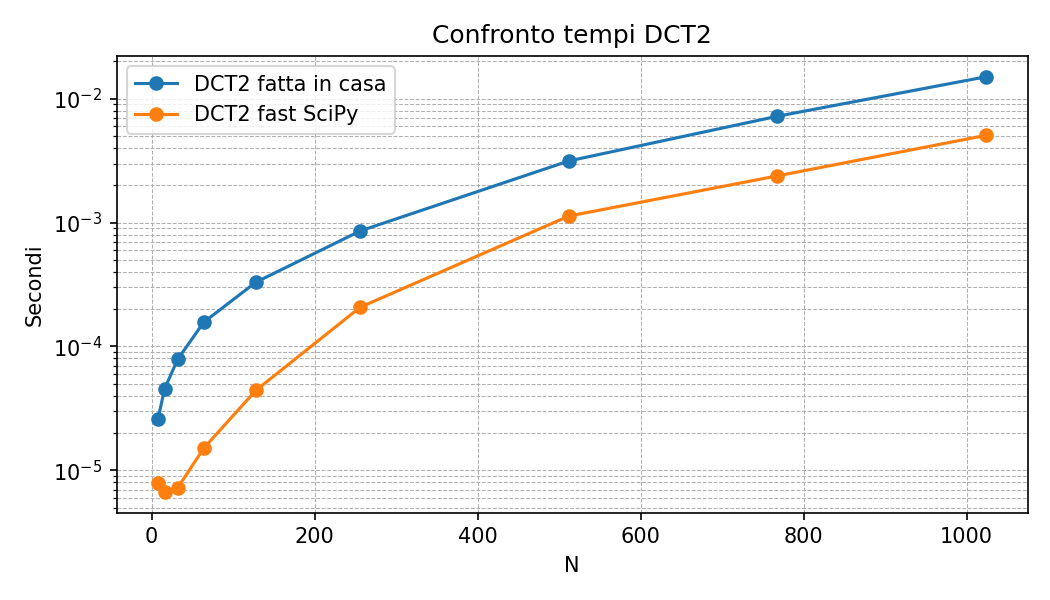
\includegraphics[width=0.92\textwidth]{figures/benchmark_dct2.png}
\caption{Tempi di esecuzione della DCT2 al variare di $N$: implementazione
\emph{custom} ($O(N^3)$) e versione FFT-based di \texttt{scipy.fft}
($O(N^2\log N)$). Scala logaritmica sulle ordinate.}
\label{fig:benchmark}
\end{figure}

I tempi misurati sono riportati nella Tabella~\ref{tab:tempi}, insieme al
rapporto fra le due implementazioni e al rapporto empirico
$t(2N)/t(N)$ per la versione \emph{custom} (che, per $O(N^3)$, dovrebbe
approssimare $8$).

\begin{table}[H]
\centering
\caption{Tempi di esecuzione (secondi) della DCT2 custom vs fast, rapporto fra
le due e rapporto $t(2N)/t(N)$ per la custom (atteso $\approx 8$ per $O(N^3)$).}
\label{tab:tempi}
\begin{tabular}{rrrrr}
\toprule
$N$ & custom (s) & fast (s) & custom/fast & $t_{\text{cust}}(2N)/t_{\text{cust}}(N)$ \\
\midrule
8    & 2.61e-05 & 7.92e-06 & 3.3  & --- \\
16   & 4.55e-05 & 6.71e-06 & 6.8  & 1.7 \\
32   & 7.86e-05 & 7.21e-06 & 10.9 & 1.7 \\
64   & 1.57e-04 & 1.51e-05 & 10.4 & 2.0 \\
128  & 3.30e-04 & 4.42e-05 & 7.5  & 2.1 \\
256  & 8.56e-04 & 2.07e-04 & 4.1  & 2.6 \\
512  & 3.15e-03 & 1.13e-03 & 2.8  & 3.7 \\
768  & 7.22e-03 & 2.38e-03 & 3.0  & --- \\
1024 & 1.50e-02 & 5.06e-03 & 3.0  & 4.8 \\
\bottomrule
\end{tabular}
\end{table}

\paragraph{Osservazioni.}
\begin{itemize}
  \item L'andamento sperimentale rispetta le predizioni teoriche: la curva
        della DCT2 \emph{custom} cresce con pendenza compatibile con $N^3$
        (raddoppiando $N$ il tempo viene moltiplicato circa per $8$); la curva
        di \texttt{scipy.fft} cresce più lentamente, compatibile con
        $N^2\log N$, e mostra piccole irregolarità dovute alla scomposizione in
        fattori primi del numero usata internamente dalla FFT.
  \item Per $N$ piccoli ($\le 32$) i tempi di entrambe le implementazioni sono
        praticamente costanti: l'\emph{overhead} delle chiamate di funzione
        domina sul costo computazionale.
  \item A partire da $N\approx 64$ i tempi crescono in modo distinguibile. Il
        rapporto $t(2N)/t(N)$ per la versione \emph{custom} si avvicina a $8$
        solo per $N$ grandi: per $N$ piccoli l'overhead costante maschera la
        scalatura cubica, che diventa visibile solo quando il costo
        computazionale domina (da $N=256$ in su il rapporto cresce
        regolarmente: $2.6\to3.7\to4.8$, verso l'asintoto $8$).
\end{itemize}

\section{Architettura del codice}\label{sec:arch}

\subsection{Algoritmo}\label{sec:algo}

Dati un intero positivo $F$ (lato del macro-blocco) e un intero
$d\in[0,\,2F-2]$ (soglia di taglio), il programma esegue i seguenti passi,
esattamente come previsto dalla traccia:
\begin{enumerate}
  \item l'immagine in scala di grigi viene divisa in blocchi quadrati $F\times F$
        partendo dall'alto a sinistra; le righe e le colonne in eccesso
        ($H\bmod F$ righe e $W\bmod F$ colonne) vengono scartate;
  \item a ciascun blocco $f$ si applica la DCT2 ortonormale (versione
        \emph{fast}) ottenendo $c = \mathrm{DCT2}(f)$;
  \item si pongono a zero tutti i coefficienti $c_{k\ell}$ con $k+\ell\ge d$,
        ossia quelli a destra dell'antidiagonale individuata da $d$;
  \item al blocco modificato si applica la IDCT2: $ff = \mathrm{IDCT2}(c)$;
  \item i pixel risultanti vengono arrotondati all'intero più vicino
        (\texttt{np.rint}) e saturati nell'intervallo $[0,255]$
        (\texttt{np.clip}), per riottenere valori ammissibili a $8$ bit;
  \item i blocchi vengono ricomposti insieme nell'ordine corretto.
\end{enumerate}

\subsection{Struttura del codice}\label{sec:struttura}

Il progetto è organizzato nei seguenti moduli:
\begin{itemize}
  \item \texttt{dct\_utils.py}: DCT/IDCT (custom e fast), maschera di taglio e
        compressione blocco-per-blocco;
  \item \texttt{run\_assignment.py}: benchmark dei tempi della prima parte e
        generazione degli esempi della seconda (griglie di compressione, grafici
        di metriche e CSV);
  \item \texttt{gui.py}: interfaccia grafica \texttt{tkinter};
  \item \texttt{test\_assignment.py}: test di validazione senza framework
        esterni;
  \item \texttt{immagini/}: immagini \texttt{.bmp} di test.
\end{itemize}

\subsection{Interfaccia grafica}\label{sec:gui}

La GUI è realizzata con \texttt{tkinter} (libreria standard di Python). Permette
di:
\begin{itemize}
  \item scegliere dal filesystem un'immagine \texttt{.bmp} in scala di grigi;
  \item impostare $F$ (ampiezza del blocco) e $d$ (soglia di taglio);
  \item eseguire la compressione e visualizzare affiancate l'immagine originale
        e quella ricostruita sui blocchi completi.
\end{itemize}
Sotto le caselle $F$ e $d$ la GUI mostra in tempo reale i valori ammessi:
dato $d$, indica il minimo $F$ necessario (poiché $d\le 2F-2$); dato $F$,
indica il range valido per $d$; se un'immagine è selezionata, indica anche il
massimo $F$ possibile per avere almeno un blocco completo. Se la coppia
corrente $(F,d)$ non è ammissibile viene segnalato esplicitamente. Se $F$ non
divide esattamente larghezza o altezza, il risultato compresso usa solo la
parte coperta da blocchi completi, mentre l'immagine originale intera rimane
visibile a sinistra; in basso viene indicata la dimensione effettivamente usata.

\section{Documentazione del codice}\label{sec:documentazione}

Il codice è documentato in modo sistematico: ogni modulo ha una \emph{docstring}
di intestazione che ne descrive lo scopo, e ogni funzione pubblica ha una
\emph{docstring} che ne specifica comportamento, argomenti (con tipo atteso),
valore di ritorno ed eccezioni sollevate. Le convenzioni seguono lo stile
\texttt{numpy}/PEP~257, con annotazioni di tipo (\emph{type hints}) sulle
firme. Di seguito si riporta la documentazione funzione per funzione.

\subsection{Modulo \texttt{dct\_utils.py}}

\paragraph{\texttt{compute\_dct\_matrix(size)}.}
Costruisce la matrice $D\in\mathbb{R}^{N\times N}$ della DCT2 ortonormale,
definita da $D_{k,i}=\alpha_k\cos\!\bigl(k\pi(2i+1)/(2N)\bigr)$ con
$\alpha_0=1/\sqrt{N}$ e $\alpha_k=\sqrt{2/N}$ per $k\ge 1$.
\begin{itemize}
  \item \emph{Input}: \texttt{size} (\texttt{int}) -- dimensione $N$.
  \item \emph{Output}: \texttt{numpy.ndarray}, shape $(N,N)$, matrice ortogonale
        ($D^{-1}=D^\top$).
  \item \emph{Eccezioni}: \texttt{ValueError} se \texttt{size}$\le 0$.
\end{itemize}

\paragraph{\texttt{dct\_1d\_fast(values)}.}
DCT monodimensionale fast con lo scaling richiesto dai test della traccia.
Wrapper di \texttt{scipy.fft.dct(..., type=2, norm='ortho')}.
\begin{itemize}
  \item \emph{Input}: \texttt{values} (array-like, shape $(N,)$).
  \item \emph{Output}: \texttt{numpy.ndarray}, shape $(N,)$, coefficienti DCT.
\end{itemize}

\paragraph{\texttt{dct\_2d\_homemade(block)}.}
DCT2 con prodotto matriciale esplicito $D\,f\,D^\top$ (costo $O(N^3)$).
\begin{itemize}
  \item \emph{Input}: \texttt{block} (array-like, shape $(N,N)$).
  \item \emph{Output}: \texttt{numpy.ndarray}, shape $(N,N)$, coefficienti DCT2.
  \item \emph{Eccezioni}: \texttt{ValueError} se l'input non è una matrice
        quadrata.
\end{itemize}

\paragraph{\texttt{dct\_2d\_fast(block)} / \texttt{idct\_2d\_fast(coefficients)}.}
DCT2 e IDCT2 fast via \texttt{scipy.fft.dctn}/\texttt{idctn} con
\texttt{type=2, norm='ortho'}.
\begin{itemize}
  \item \emph{Input}: array 2D (shape $(N,N)$).
  \item \emph{Output}: array 2D, trasformato / ricostruito.
  \item \emph{Eccezioni}: \texttt{ValueError} se l'input non è bidimensionale.
\end{itemize}

\paragraph{\texttt{frequency\_keep\_mask(block\_size, cutoff)}.}
Maschera booleana di taglio: \texttt{True} dove $k+\ell<d$ (conservato),
\texttt{False} dove $k+\ell\ge d$ (azzerato). Costruita vettorialmente con
\texttt{np.indices}.
\begin{itemize}
  \item \emph{Input}: \texttt{block\_size} (\texttt{int}, $=F$), \texttt{cutoff}
        (\texttt{int}, $=d$).
  \item \emph{Output}: \texttt{numpy.ndarray} di \texttt{bool}, shape $(F,F)$.
  \item \emph{Eccezioni}: \texttt{ValueError} se $F\le 0$ o $d\notin[0,2F-2]$.
\end{itemize}

\paragraph{\texttt{compress\_image\_array(image, block\_size, cutoff)}.}
Esegue l'intera procedura di compressione/decompressione blocco per blocco.
\begin{itemize}
  \item \emph{Input}: \texttt{image} (array 2D scala di grigi), \texttt{block\_size}
        (\texttt{int}), \texttt{cutoff} (\texttt{int}).
  \item \emph{Output}: tupla \texttt{(original, compressed)}: porzione
        croppata dell'originale e immagine ricomposta, entrambe \texttt{uint8},
        shape $(H_c,W_c)$ con $H_c=\lfloor H/F\rfloor F$, $W_c=\lfloor W/F\rfloor F$.
  \item \emph{Eccezioni}: \texttt{ValueError} se l'input non è 2D, se $F/d$
        non sono ammissibili, o se l'immagine è più piccola del blocco.
\end{itemize}

\paragraph{\texttt{load\_bmp\_grayscale(path)} / \texttt{save\_grayscale\_image(path, image)}.}
Caricano/salvano un'immagine \texttt{.bmp} in scala di grigi come array
\texttt{uint8} 2D, via \texttt{Pillow}.
\begin{itemize}
  \item \emph{Eccezioni}: \texttt{ValueError} se il file non ha estensione
        \texttt{.bmp}.
\end{itemize}

\paragraph{\texttt{time\_function(function, *args, repeats=3)}.}
Misura il tempo di esecuzione di una funzione restituendo il \emph{minimo} su
\texttt{repeats} chiamate (per ridurre il rumore), via
\texttt{time.perf\_counter}.
\begin{itemize}
  \item \emph{Output}: \texttt{float}, tempo minimo in secondi.
\end{itemize}

\subsection{Modulo \texttt{run\_assignment.py}}

\paragraph{\texttt{main()}.}
Parsa gli argomenti da riga di comando, esegue il benchmark dei tempi (con
\texttt{--size} ripetibile, \texttt{--repeats}) e, salvo \texttt{--no-examples},
genera per ogni immagine una griglia di compressioni, un grafico di metriche e
un CSV in \texttt{results/examples/}.

\paragraph{\texttt{run\_benchmark(sizes, repeats)}.}
Ciclo di misura: per ogni $N$ genera una matrice casuale $N\times N$ (seed
fisso per riproducibilità), cronometra \texttt{dct\_2d\_homemade} e
\texttt{dct\_2d\_fast} e restituisce le righe del CSV.

\paragraph{\texttt{calculate\_metrics(original, compressed)}.}
Calcola MSE e PSNR (dB) fra originale e compressa:
$\mathrm{PSNR}=20\log_{10}(255/\sqrt{\mathrm{MSE}})$, con $\mathrm{PSNR}=\infty$
se $\mathrm{MSE}=0$.

\paragraph{\texttt{calculate\_compression\_ratio(block\_size, cutoff)}.}
Restituisce la frazione di coefficienti conservati
$n_{\text{kept}}/F^2$ tramite \texttt{frequency\_keep\_mask}.

\paragraph{Funzioni di plotting.}
\texttt{plot\_benchmark} (semilog-$y$ dei tempi), \texttt{save\_compression\_grid}
(griglia delle immagini compresse con PSNR nei titoli),
\texttt{save\_informative\_plots} (PSNR vs $d$ e PSNR vs \% coefficienti),
\texttt{write\_image\_metrics\_csv} e \texttt{write\_benchmark\_csv}
(serializzazione CSV).

\subsection{Modulo \texttt{gui.py}}

\paragraph{Classe \texttt{CompressionApp}.}
Finestra principale; costruisce i widget (pulsante \emph{Scegli BMP}, caselle
$F$ e $d$, pulsante \emph{Comprimi}, due canvas per originale/compressa) e gestisce
gli eventi. Mantiene riferimenti alle \texttt{PhotoImage} per evitare la
rimozione da parte del \emph{garbage collector}.

\paragraph{Metodi principali.}
\texttt{choose\_image} (apre il dialog di selezione e carica),
\texttt{compress} (valida $F,d$, esegue \texttt{build\_compression\_preview},
aggiorna le anteprime), \texttt{update\_parameter\_help} (suggerimenti live su
$F$/$d$), \texttt{render\_previews}/\texttt{draw\_image} (disegno adattato al
canvas).

\paragraph{Funzioni ausiliarie.}
\texttt{fit\_preview\_size(image\_size, available\_size)} (ridimensiona
mantenendo le proporzioni entro l'area disponibile),
\texttt{array\_to\_photo} (array $\to$ \texttt{PhotoImage}),
\texttt{load\_original\_preview}, \texttt{build\_compression\_preview}
(orchestra caricamento + compressione + messaggio di stato),
\texttt{describe\_parameter\_hints} (calcola i testi di suggerimento sui limiti
ammissibili di $F$ e $d$). Tutti gli errori (file non valido, $F/d$ non interi,
$d$ fuori range, $F$ più grande dell'immagine) sono segnalati all'utente con
\texttt{messagebox} senza arrestare il programma.

\section{Esperimenti}\label{sec:esperimenti}

Su ciascuna immagine della cartella \texttt{immagini/} sono state testate
$12$ coppie di parametri: quattro con $F=8$, quattro con $F=16$ e quattro con
$F=32$, a soglie crescenti, per studiare sia l'effetto del taglio a parità di
dimensione del blocco sia l'effetto della dimensione del blocco. Per ogni
configurazione sono stati salvati una griglia di compressioni, un grafico di
metriche (PSNR vs $d$ e PSNR vs percentuale di coefficienti mantenuti) e un
CSV numerico. La qualità è misurata con MSE e PSNR:
\[
\mathrm{MSE} = \frac{1}{n}\sum_i (x_i - \hat x_i)^2, \qquad
\mathrm{PSNR} = 20\log_{10}\!\left(\frac{255}{\sqrt{\mathrm{MSE}}}\right)\ \text{dB}.
\]

Le immagini di test si dividono in due famiglie:
\begin{enumerate}
  \item immagini sintetiche regolari: scacchiere a varie risoluzioni
        ($20\times20$, $40\times40$, \dots, $640\times640$), un gradiente
        orizzontale (\texttt{gradient}) e un carattere a contrasto pieno
        (\texttt{prova}, una \guillemotleft C\guillemotright{} su sfondo scuro);
  \item fotografie reali: \texttt{bridge}, \texttt{cathedral}, \texttt{deer},
        \texttt{shoe}, \texttt{tonypitony}.
\end{enumerate}

\subsection{Immagini regolari: gradiente}

Il gradiente è un caso ideale per la DCT: i coefficienti si concentrano quasi
tutti su poche basi a bassa frequenza, e tagliarne una larga maggioranza ha
effetto trascurabile. Alla massima soglia $d=14$ (con $F=8$) la ricostruzione è
esatta (MSE$=0$, PSNR$=\infty$); anche conservando solo il $4.7\%$ dei
coefficienti ($d=2$) la PSNR resta sopra i $54$~dB. La
Figura~\ref{fig:gradient} mostra la griglia di compressioni, la
Figura~\ref{fig:gradient_metrics} le metriche.

\begin{figure}[H]
\centering
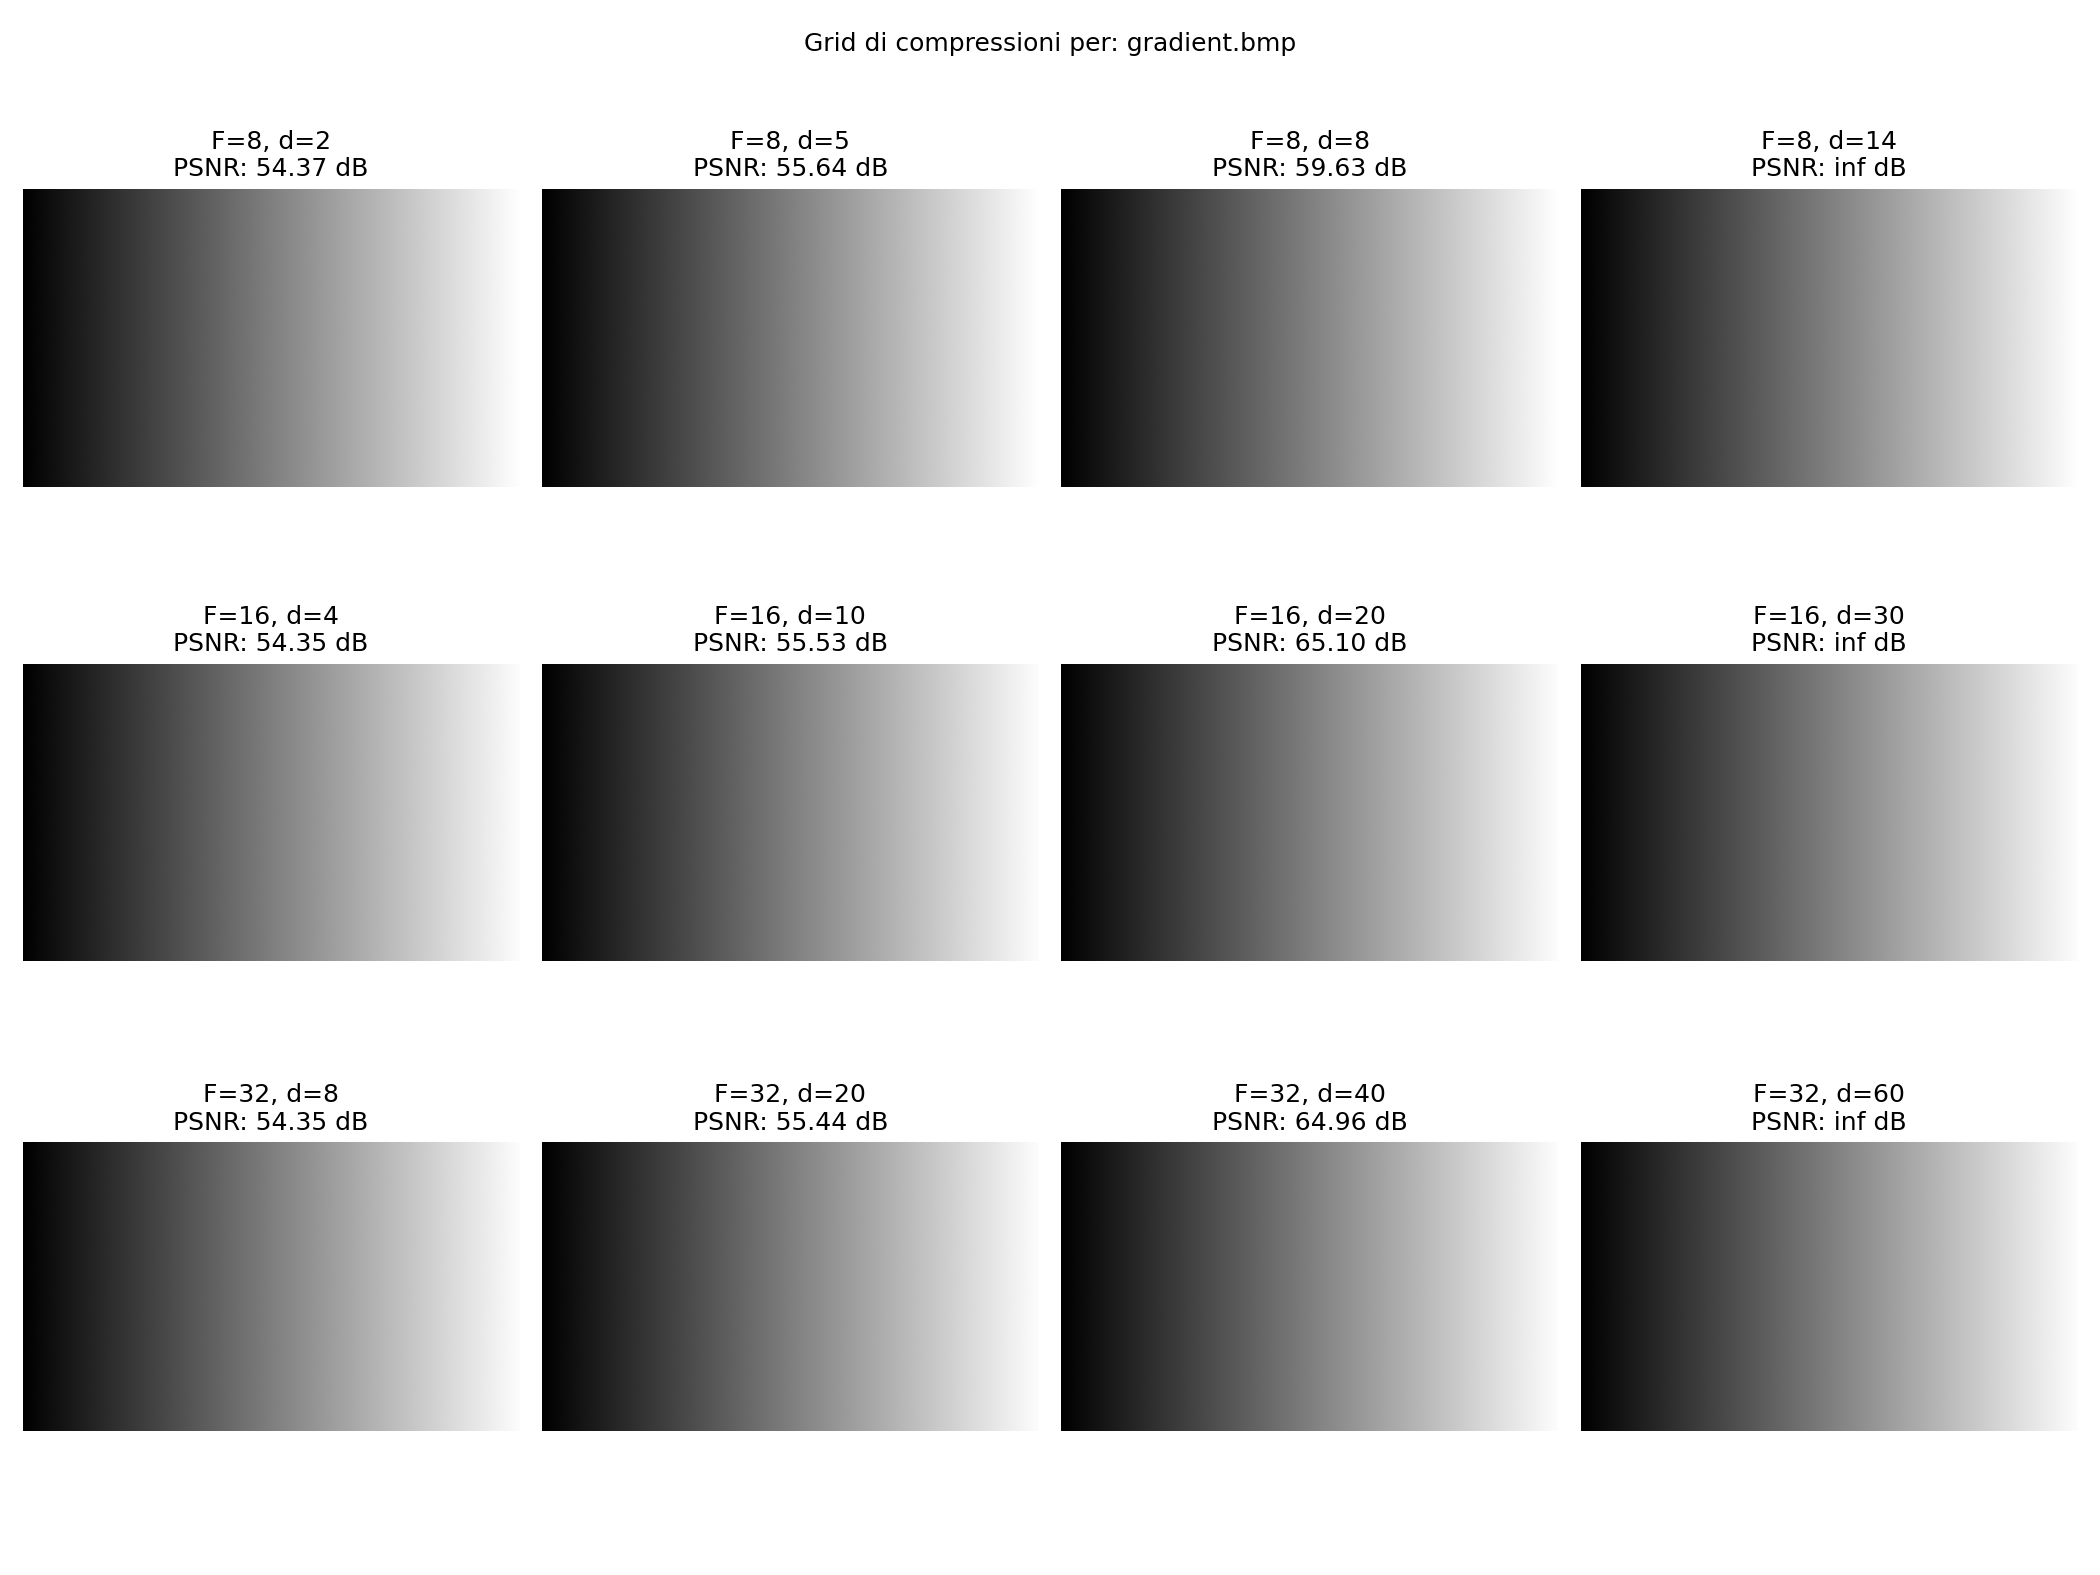
\includegraphics[width=0.85\textwidth]{figures/gradient_grid.png}
\caption{Compressione del gradiente a varie $(F,d)$. Immagine perfettamente
liscia: anche con pochissimi coefficienti la qualità resta eccellente.}
\label{fig:gradient}
\end{figure}

\begin{figure}[H]
\centering
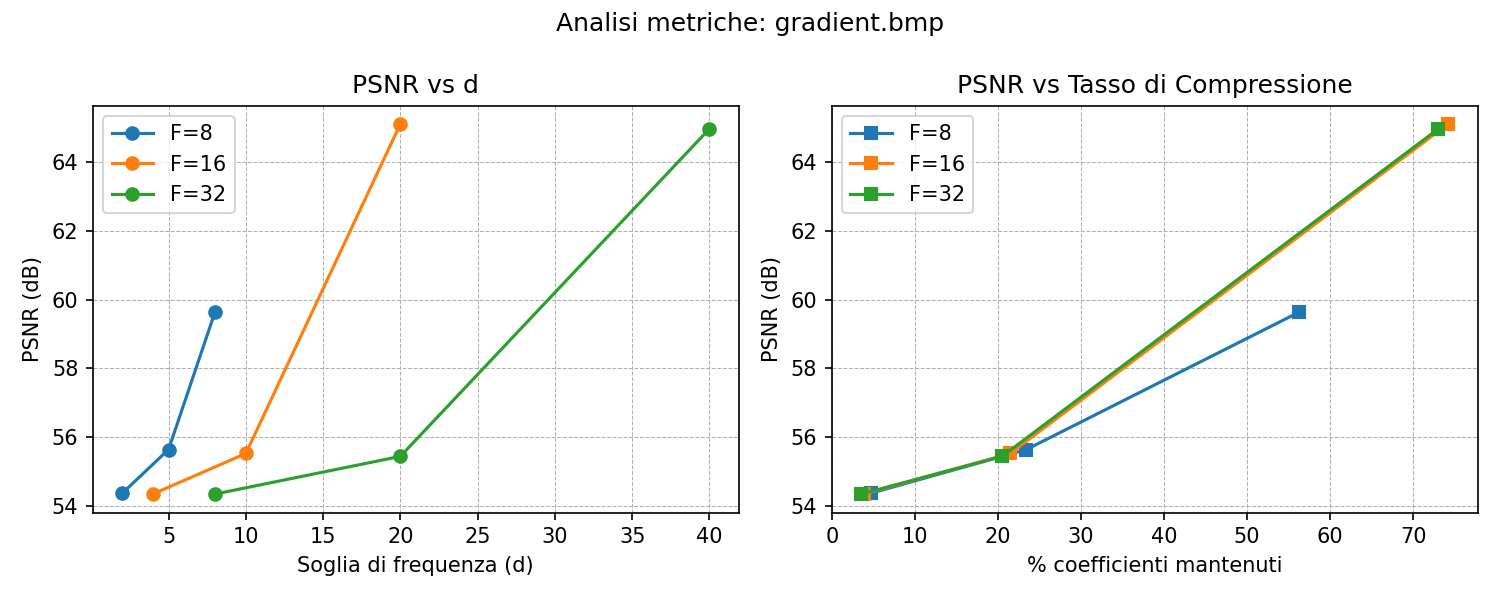
\includegraphics[width=0.80\textwidth]{figures/gradient_metrics.png}
\caption{Metriche sul gradiente: PSNR vs $d$ (sinistra) e vs \% coefficienti
mantenuti (destra).}
\label{fig:gradient_metrics}
\end{figure}

\subsection{Immagini con bordi netti: scacchiere e lettera \guillemotleft C\guillemotright}

Nelle immagini con bordi netti i coefficienti DCT non decadono rapidamente:
tagliarli equivale a troncare la serie di Fourier in prossimità di un salto, ed
è qui che compare il fenomeno di Gibbs (oscillazioni spurie localizzate vicino
al bordo). L'effetto è particolarmente evidente sulla scacchiera $320\times320$
con $F=8$, $d=2$: la PSNR scende a $9.9$~dB e la ricostruzione mostra un
artefatto pesante (Figura~\ref{fig:checker}); con blocchi grandi ($F=32$) si
somma un evidente effetto a blocchi. La lettera \guillemotleft C\guillemotright{}
(\texttt{prova}) mostra lo stesso fenomeno su un contorno curvo
(Figura~\ref{fig:prova}).

\begin{figure}[H]
\centering
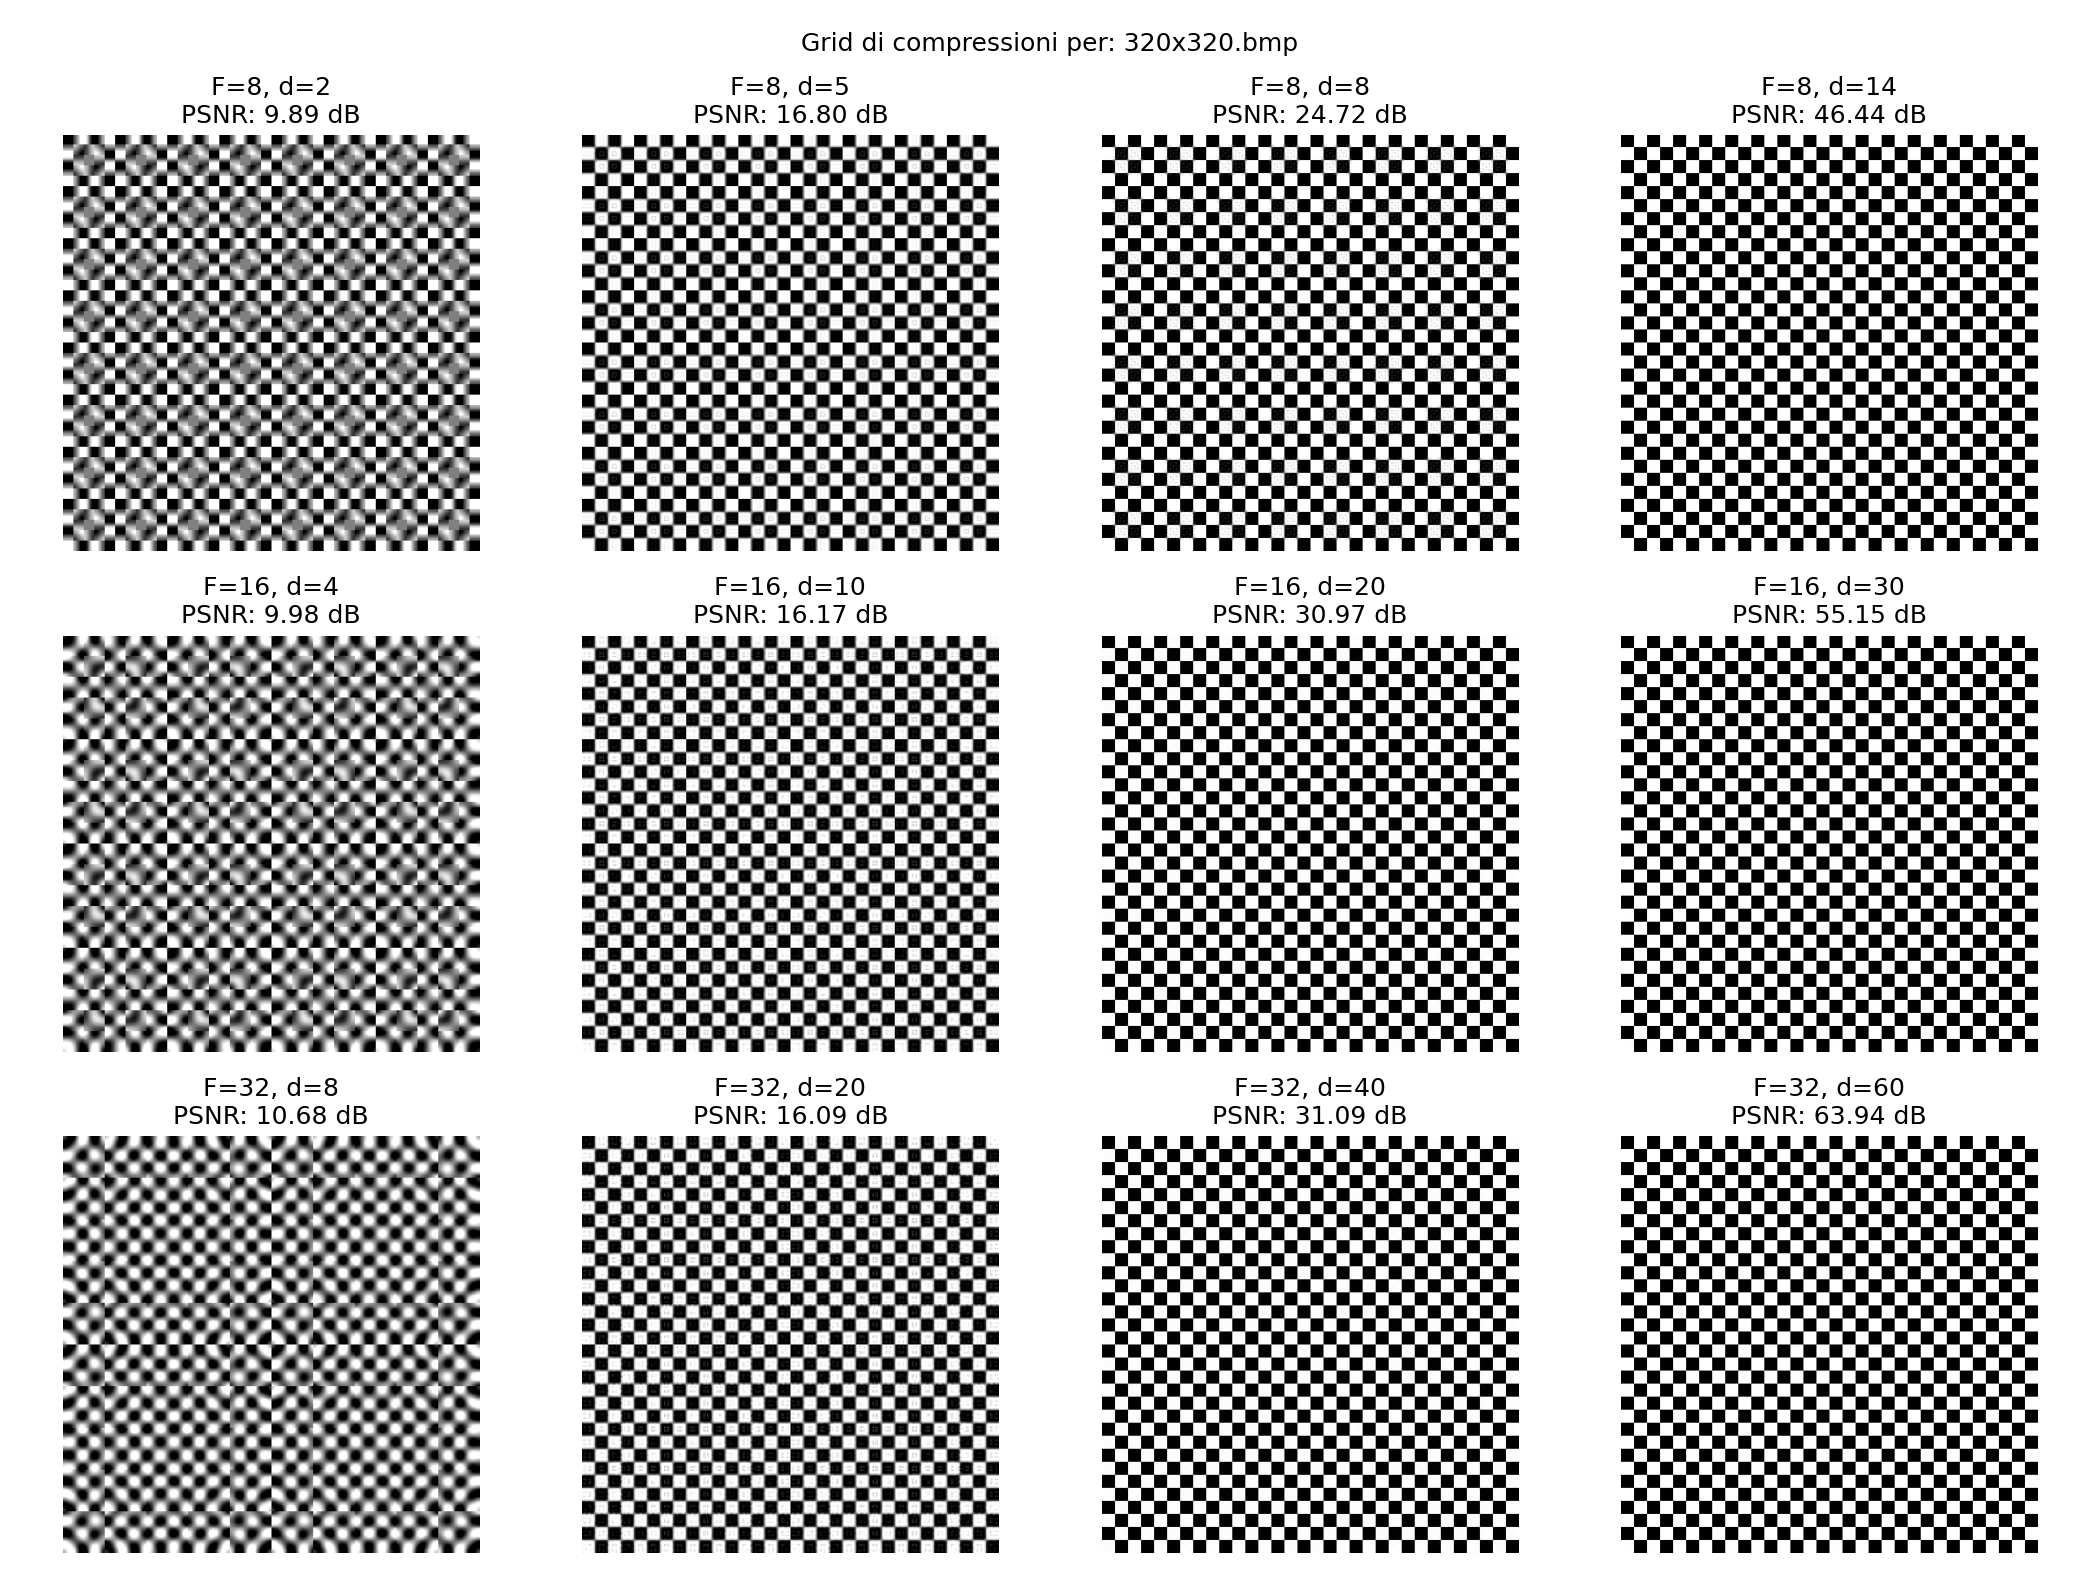
\includegraphics[width=0.85\textwidth]{figures/320x320_grid.png}
\caption{Scacchiera $320\times320$: in presenza di discontinuità nette il
taglio delle alte frequenze produce l'effetto di Gibbs; con $F=32$ si aggiunge
un artefatto a blocchi.}
\label{fig:checker}
\end{figure}

\begin{figure}[H]
\centering
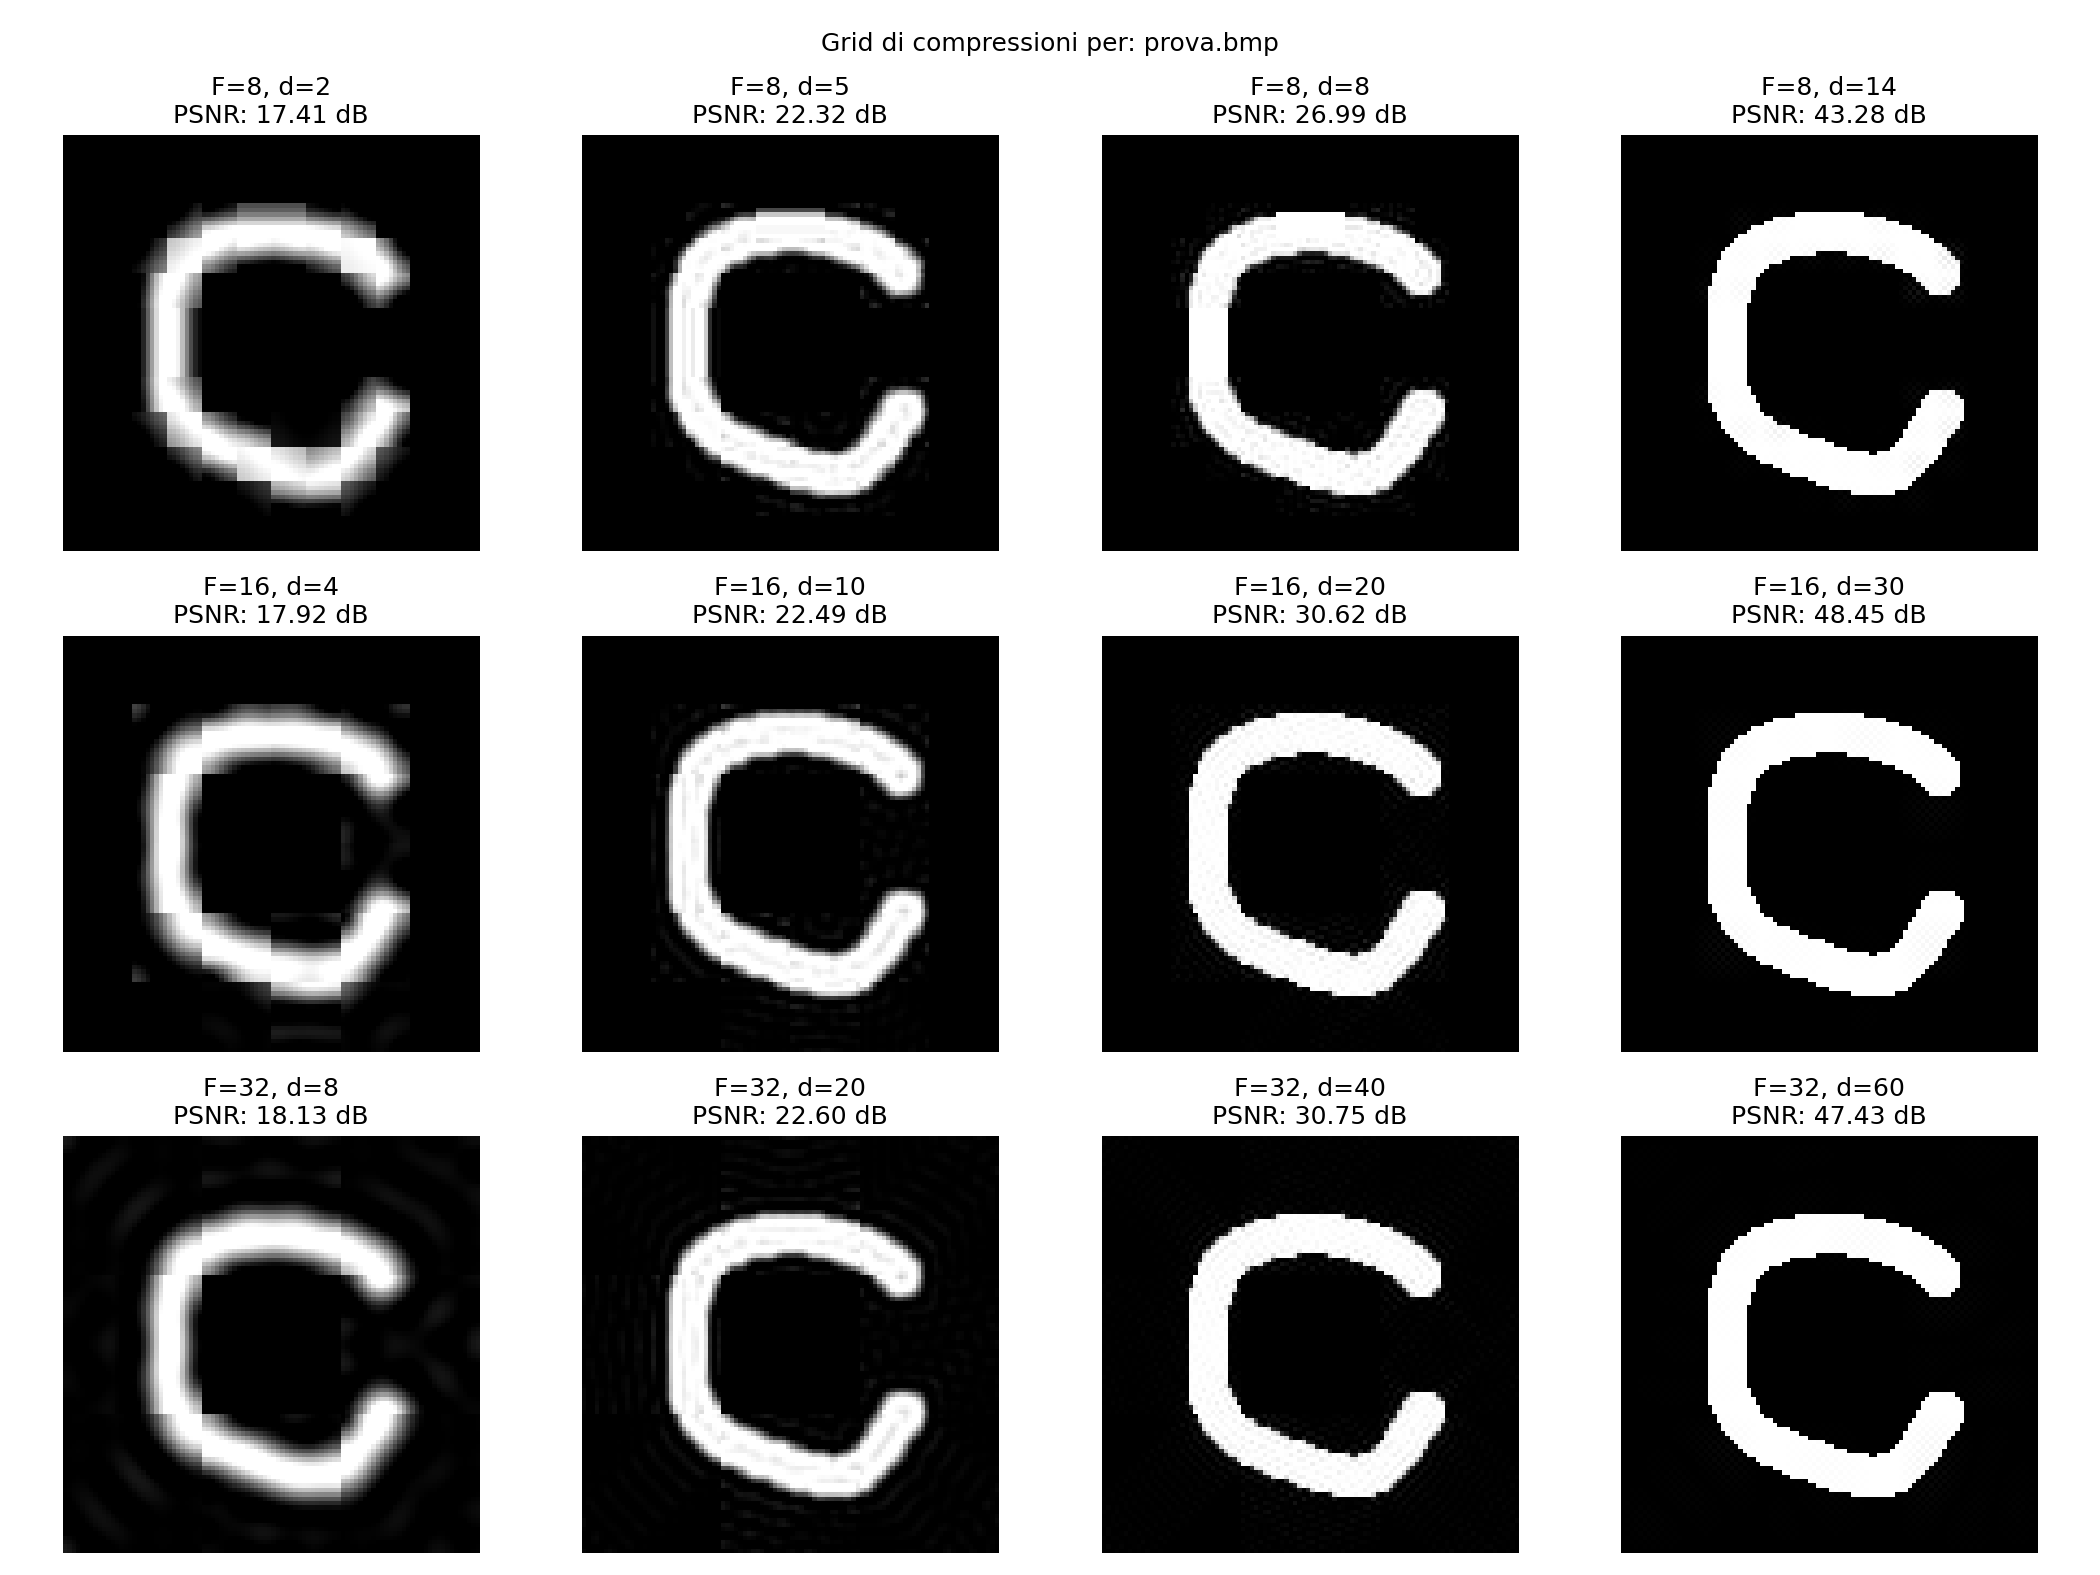
\includegraphics[width=0.78\textwidth]{figures/prova_grid.png}
\caption{Lettera \guillemotleft C\guillemotright{} (\texttt{prova}): il bordo
curvo perde nitidezza al ridursi di $d$; con $F=8$, $d=2$ la PSNR scende a
$17.4$~dB.}
\label{fig:prova}
\end{figure}

\subsubsection{Confronto fra risoluzioni (scacchiere)}

Le scacchiere ($20\times20$, $40\times40$, \dots, $640\times640$) mostrano
valori identici sulle righe $F=8$: ciò avviene perché la scacchiera ha celle di
lato divisore di $8$, dunque il pattern si ripete identico in ogni blocco
$8\times8$. La Tabella~\ref{tab:checker} lo dimostra: le colonne $F=8$ sono
identiche per tutte le risoluzioni. Le righe $F=16$ e $F=32$ presentano invece
piccole differenze, perché cambia il rapporto fra periodo del pattern e
dimensione del blocco. L'immagine $20\times20$ (in realtà $16\times16$) è più
piccola del blocco $32\times32$: la configurazione $F=32$ non viene applicata
(riportata come \texttt{--}). La Figura~\ref{fig:checker_res} mostra le
scacchiere a tre risoluzioni affiancate.

\begin{table}[H]
\centering
\caption{PSNR [dB] sulle scacchiere a varie risoluzioni, $F=8$. I valori sono
identici perché il pattern si ripete uguale in ogni blocco $8\times8$.}
\label{tab:checker}
\begin{tabular}{lrrrr}
\toprule
Immagine & $d=2$ & $d=5$ & $d=8$ & $d=14$ \\
\midrule
$20\times20$  & 10.7 & 17.7 & 26.5 & 51.1 \\
$40\times40$  & 9.9  & 16.8 & 24.7 & 46.4 \\
$80\times80$  & 9.9  & 16.8 & 24.7 & 46.4 \\
$160\times160$& 9.9  & 16.8 & 24.7 & 46.4 \\
$320\times320$& 9.9  & 16.8 & 24.7 & 46.4 \\
$640\times640$& 9.9  & 16.8 & 24.7 & 46.4 \\
\bottomrule
\end{tabular}
\end{table}

\begin{figure}[H]
\centering
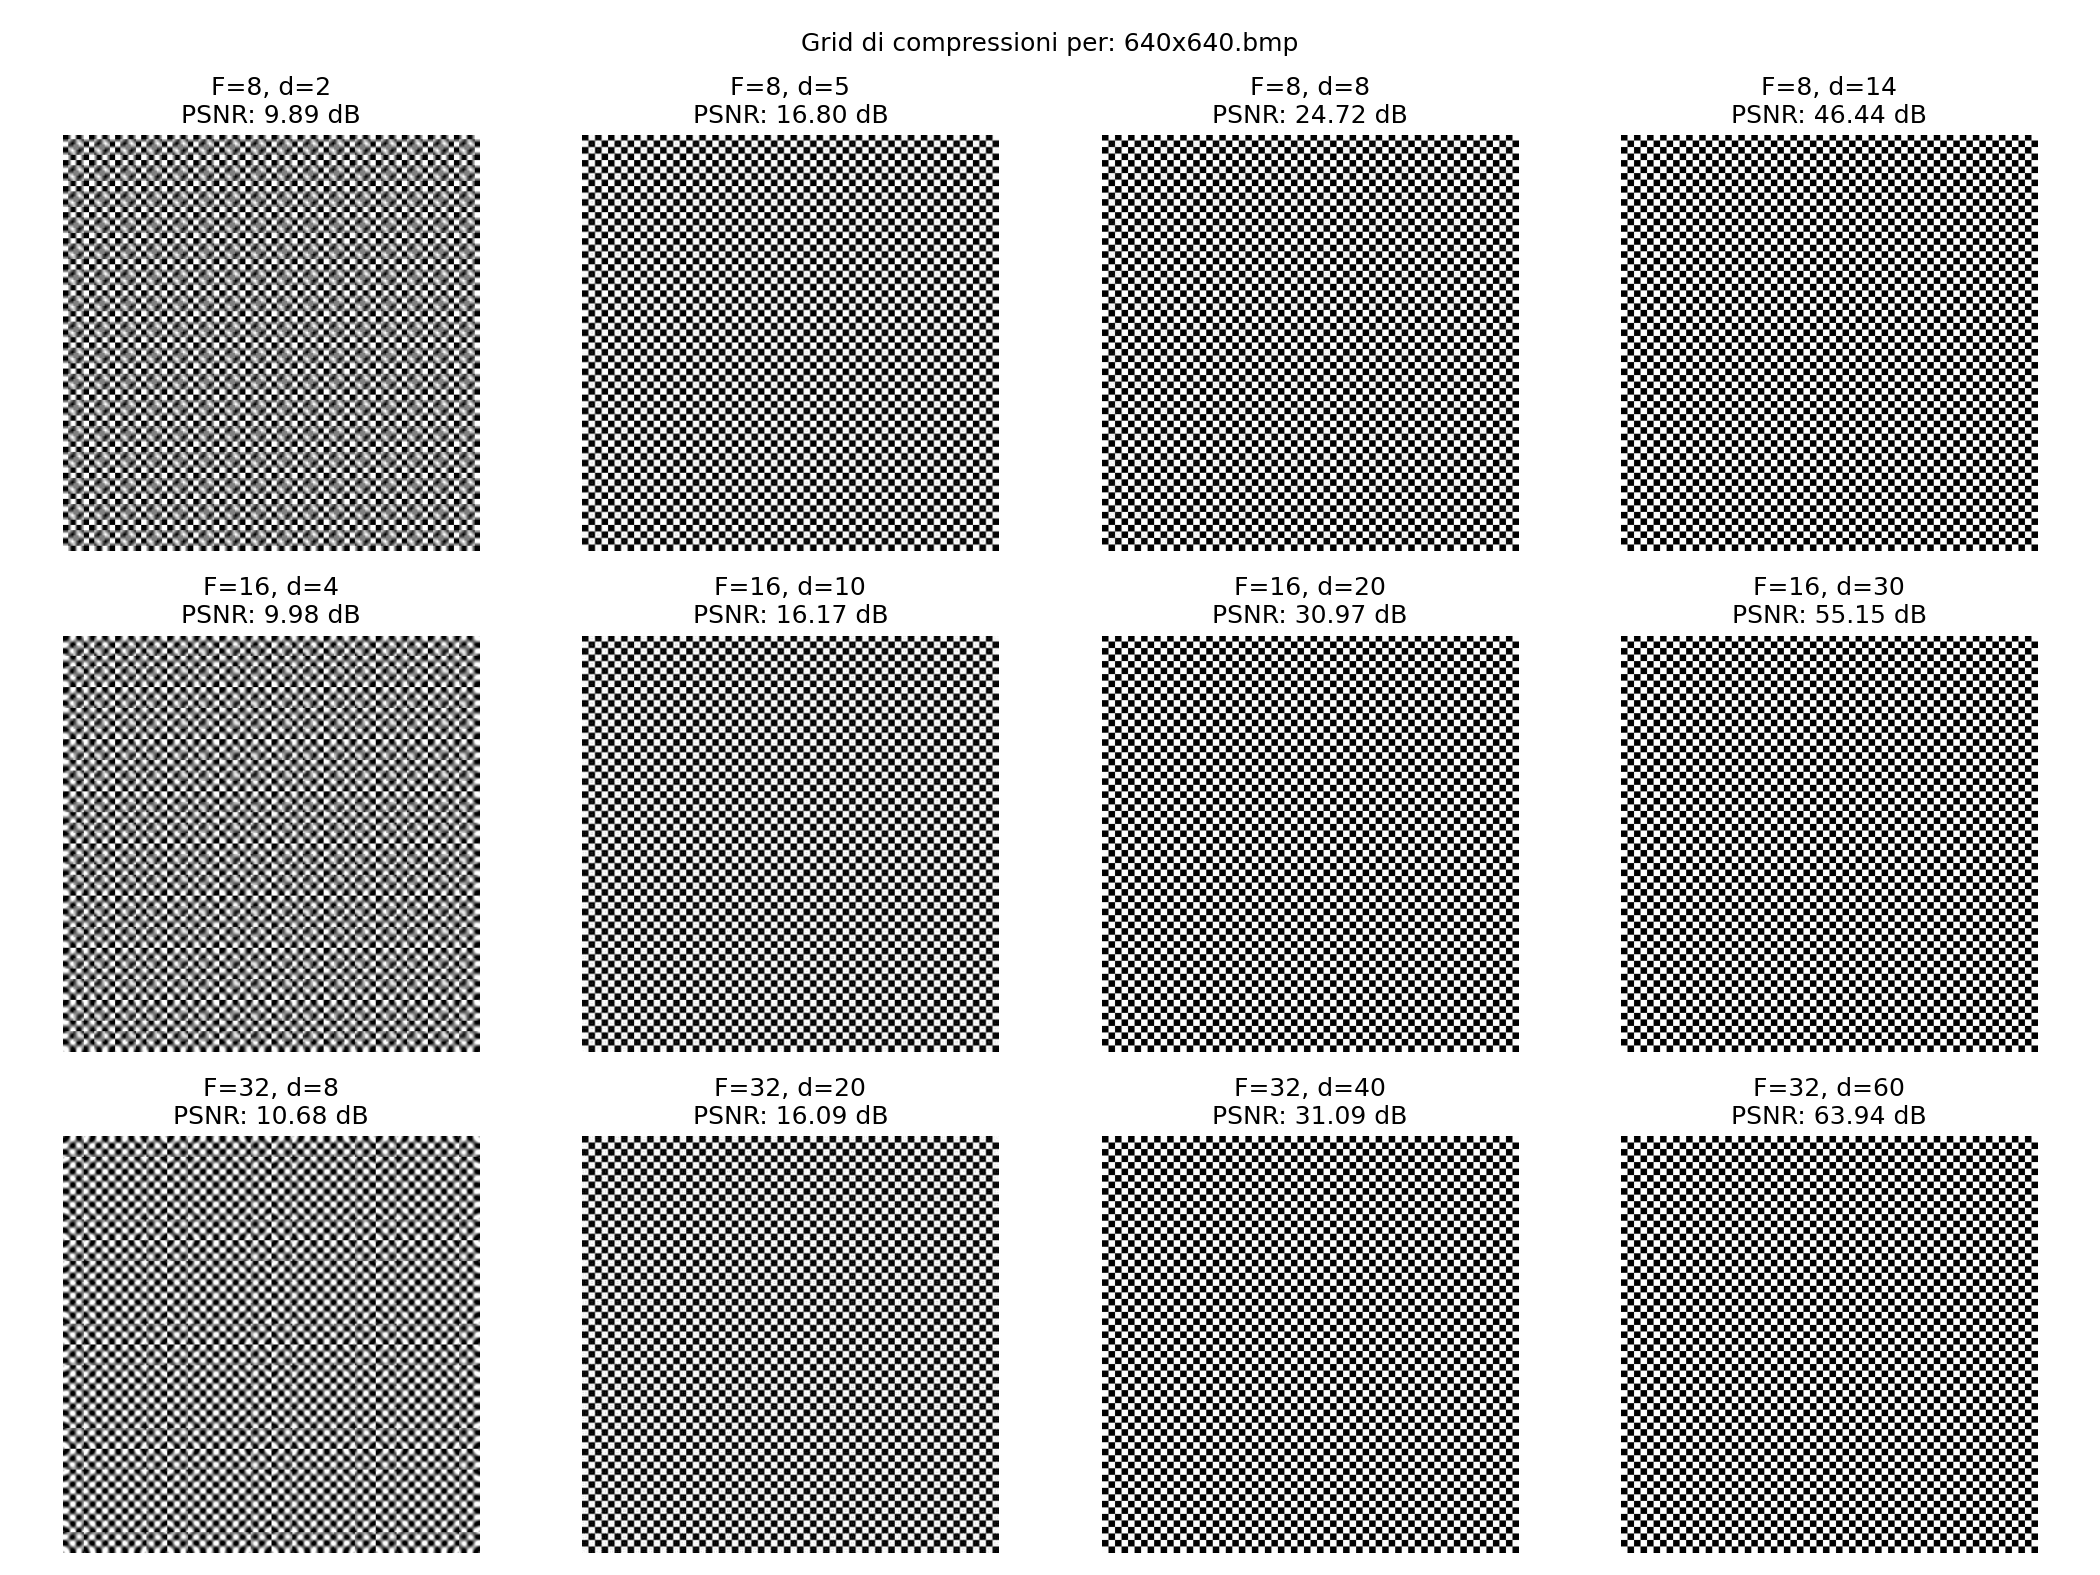
\includegraphics[width=0.70\textwidth]{figures/640x640_grid.png}
\caption{Scacchiera $640\times640$, $F=8$/$16$/$32$ a $d$ crescenti: stesso
artefatto di Gibbs della $320\times320$, a conferma dell'invarianza rispetto
alla risoluzione a parità di $F=8$.}
\label{fig:checker_res}
\end{figure}

\subsection{Fotografie reali}

Sulle fotografie reali i risultati sono molto migliori che sulle scacchiere,
perché le immagini naturali sono più localmente uniformi: all'interno di un
blocco $8\times8$ tipico la variazione di intensità è quasi sempre piccola.
La Tabella~\ref{tab:psnr} riporta i valori di PSNR selezionati; la
Tabella~\ref{tab:dati} (in fondo, \emph{longtable}) riporta l'elenco completo
di MSE, PSNR e percentuale di coefficienti mantenuti per ogni configururazione.
Ad alto taglio ($d=14$ con $F=8$) tutte le foto reali superano $63$~dB
(qualità eccellente), e anche al taglio più aggressivo ($d=2$, conservando solo
il $4.7\%$ dei coefficienti) si mantengono tra $22$ e $30$~dB, una qualità
ancora buona. Le Figure~\ref{fig:deer}--\ref{fig:tonypitony} mostrano le griglie
di compressioni e i grafici di metriche per le foto reali.

\begin{table}[H]
\centering
\caption{PSNR [dB] misurato sulle immagini al variare di $(F,d)$: foto reali
(above) e rappresentative sintetiche (below).}
\label{tab:psnr}
\small
\begin{tabular}{lrrrrrr}
\toprule
& \multicolumn{3}{c}{$F=8$} & \multicolumn{1}{c}{$F=16$} & \multicolumn{1}{c}{$F=32$} \\
\cmidrule(lr){2-4}\cmidrule(lr){5-5}\cmidrule(lr){6-6}
Immagine & $d=2$ & $d=5$ & $d=8$ & $d=14$ & $d=10$ & $d=20$ \\
\midrule
deer       & 29.6 & 35.8 & 42.0 & 66.1 & 35.9 & 47.0 \\
bridge     & 28.7 & 37.5 & 44.0 & 68.3 & 37.6 & 48.7 \\
cathedral  & 30.7 & 39.1 & 45.5 & 69.1 & 39.3 & 49.7 \\
shoe       & 22.6 & 31.0 & 41.0 & 76.6 & 31.3 & 49.1 \\
tonypitony & 26.0 & 32.5 & 40.3 & 63.5 & 32.5 & 45.4 \\
\midrule
gradient   & 54.4 & 55.6 & 59.6 & $\infty$ & 55.5 & 65.1 \\
prova (C)  & 17.4 & 22.3 & 27.0 & 43.3 & 22.5 & 30.6 \\
320x320    & 9.9  & 16.8 & 24.7 & 46.4 & 16.2 & 31.0 \\
\bottomrule
\end{tabular}
\end{table}

\begin{figure}[H]
\centering
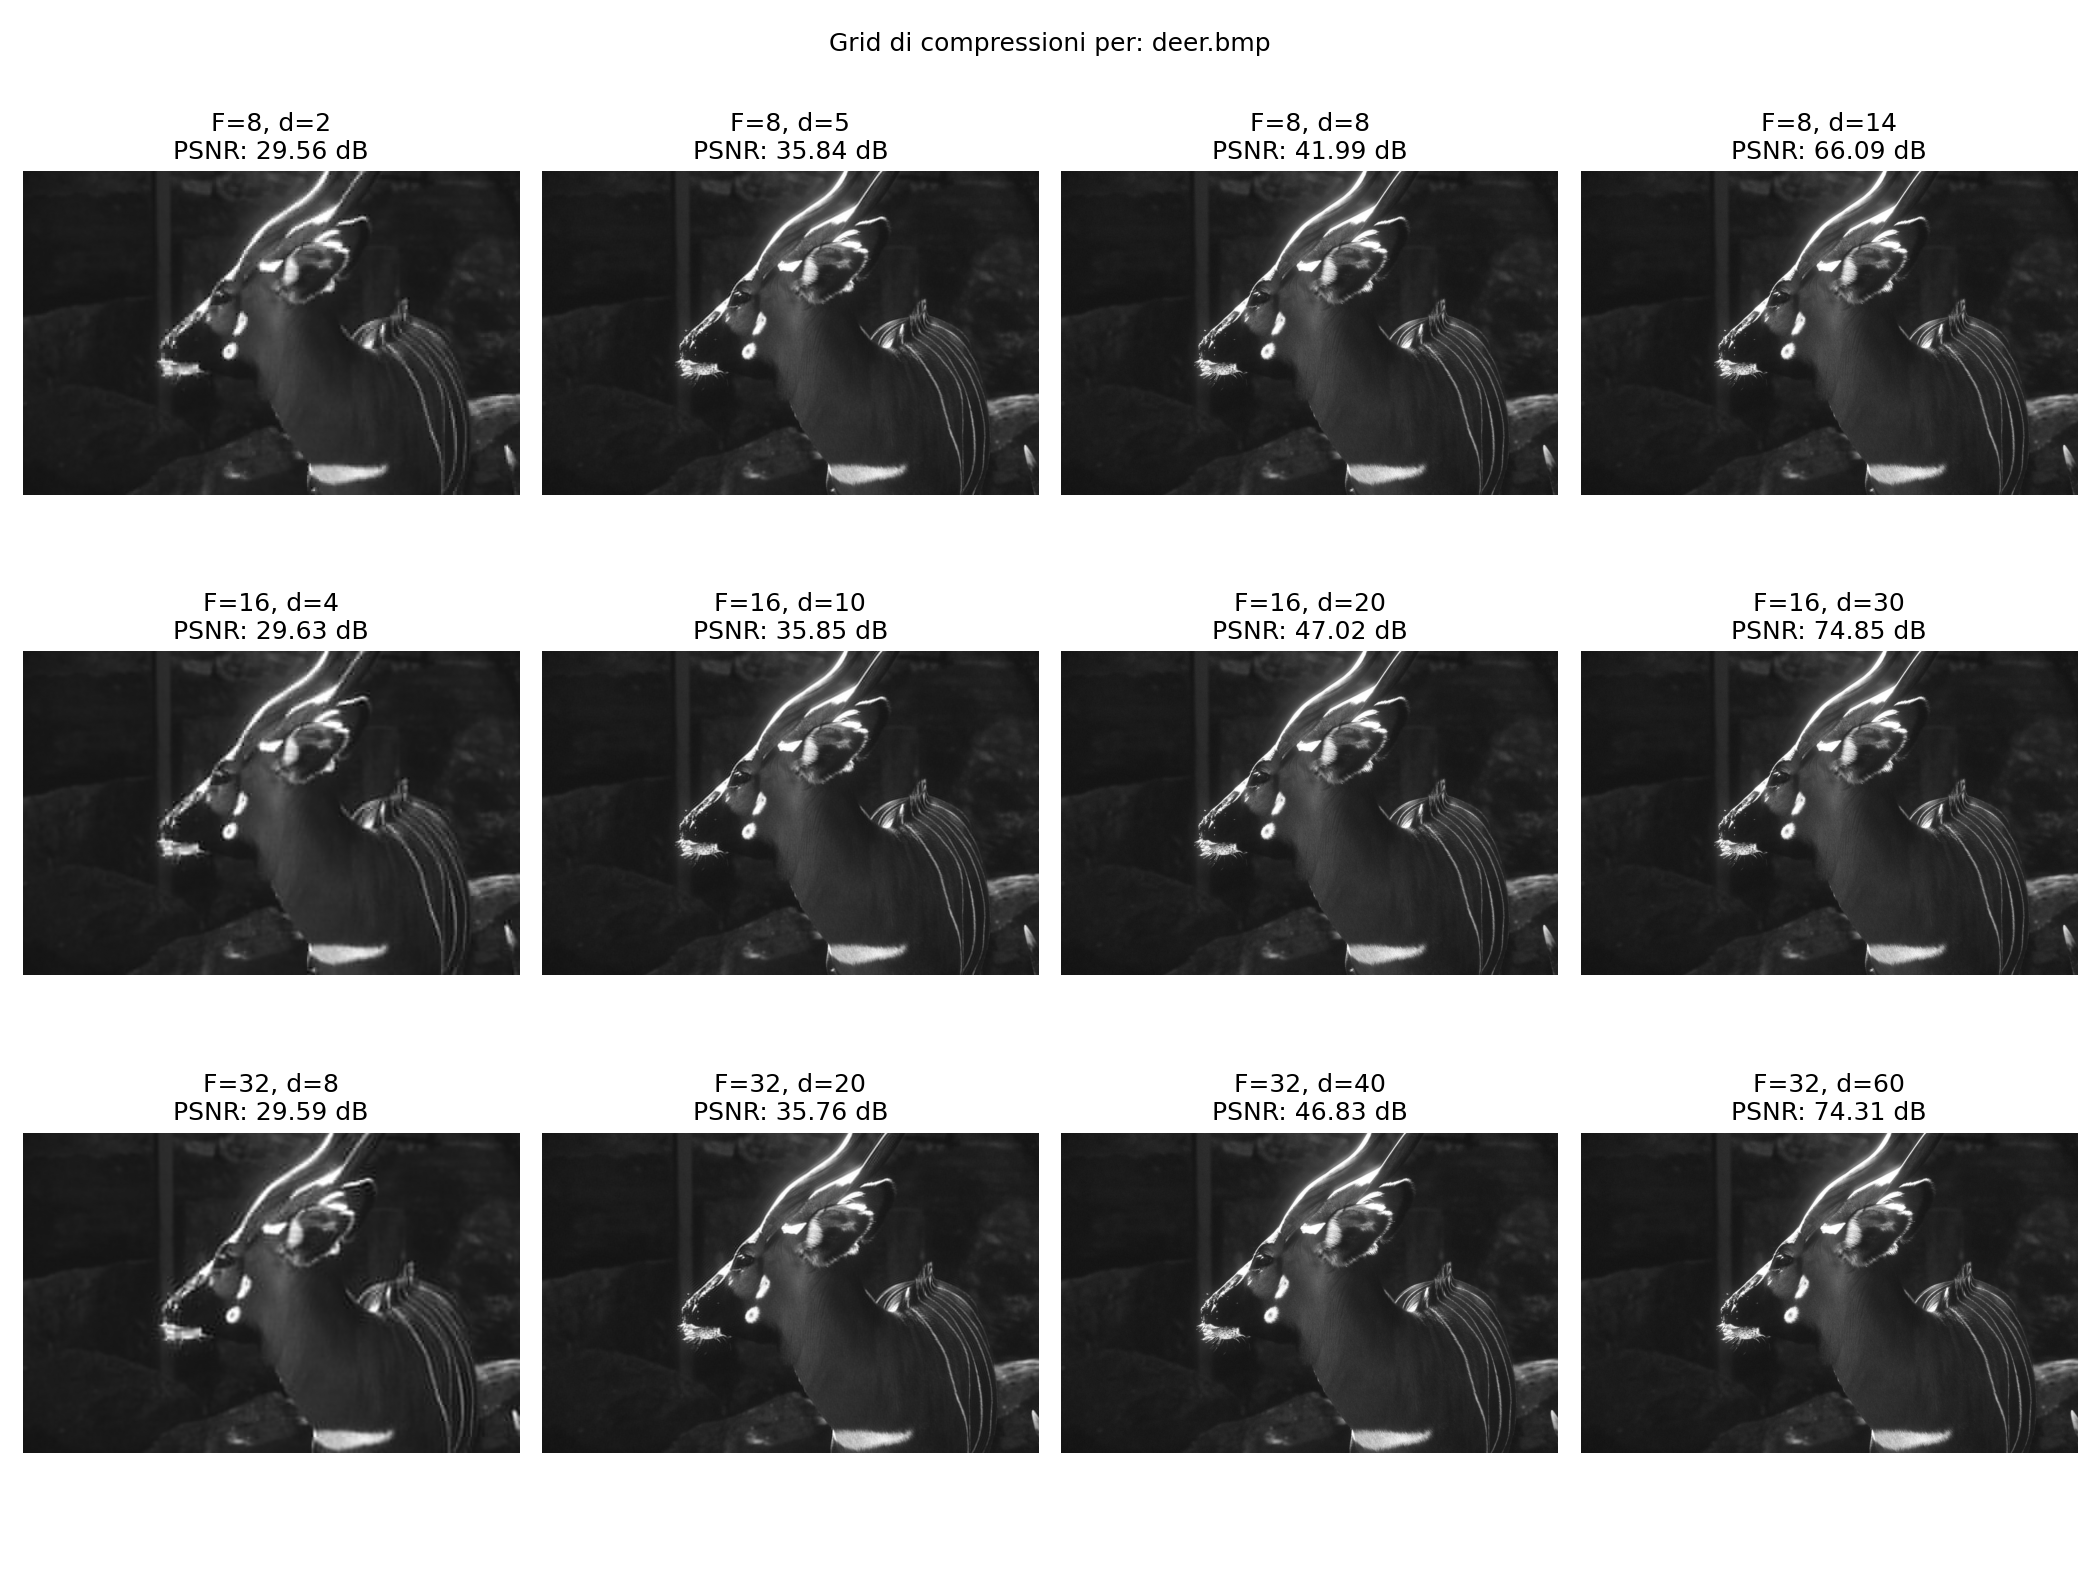
\includegraphics[width=0.85\textwidth]{figures/deer_grid.png}
\caption{Fotografia reale \texttt{deer}: a $d=14$ la ricostruzione è
indistinguibile dall'originale; anche con pochi coefficienti la qualità visiva
rimane accettabile.}
\label{fig:deer}
\end{figure}

\begin{figure}[H]
\centering
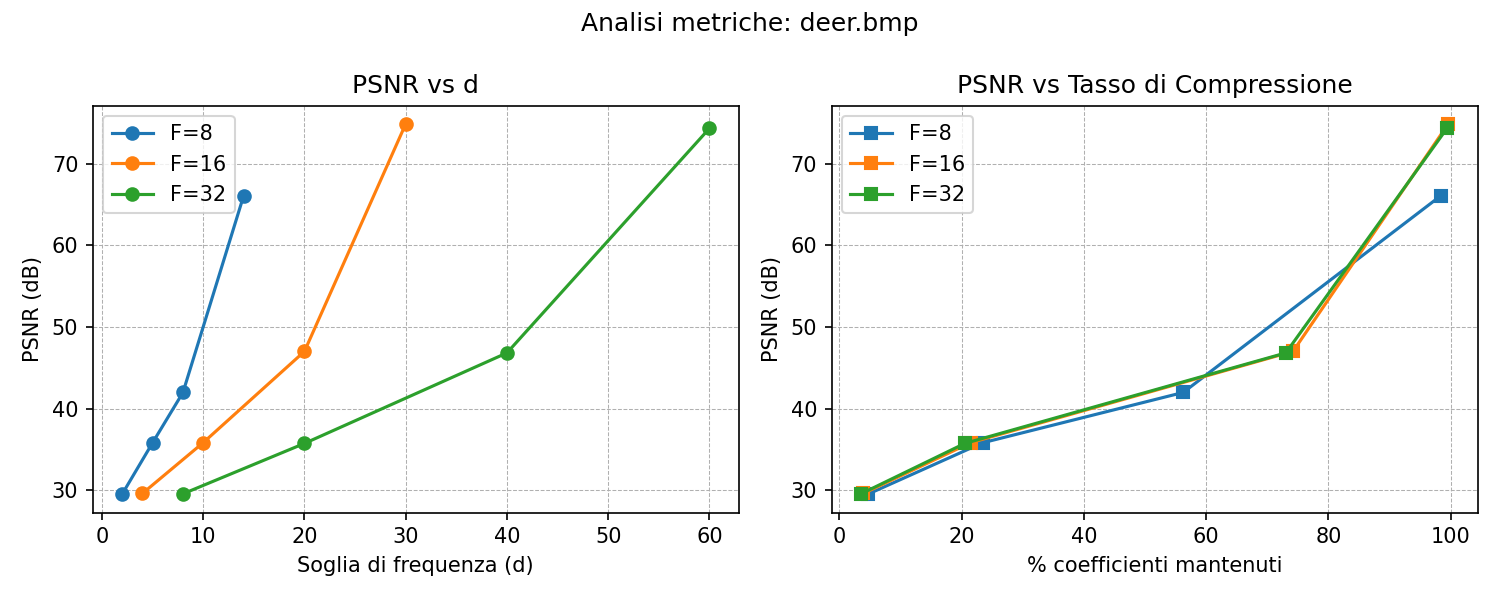
\includegraphics[width=0.78\textwidth]{figures/deer_metrics.png}
\caption{Metriche su \texttt{deer}: PSNR vs $d$ (sinistra) e vs \% coefficienti
mantenuti (destra).}
\label{fig:deer_metrics}
\end{figure}

\begin{figure}[H]
\centering
\begin{subfigure}{0.49\textwidth}\centering
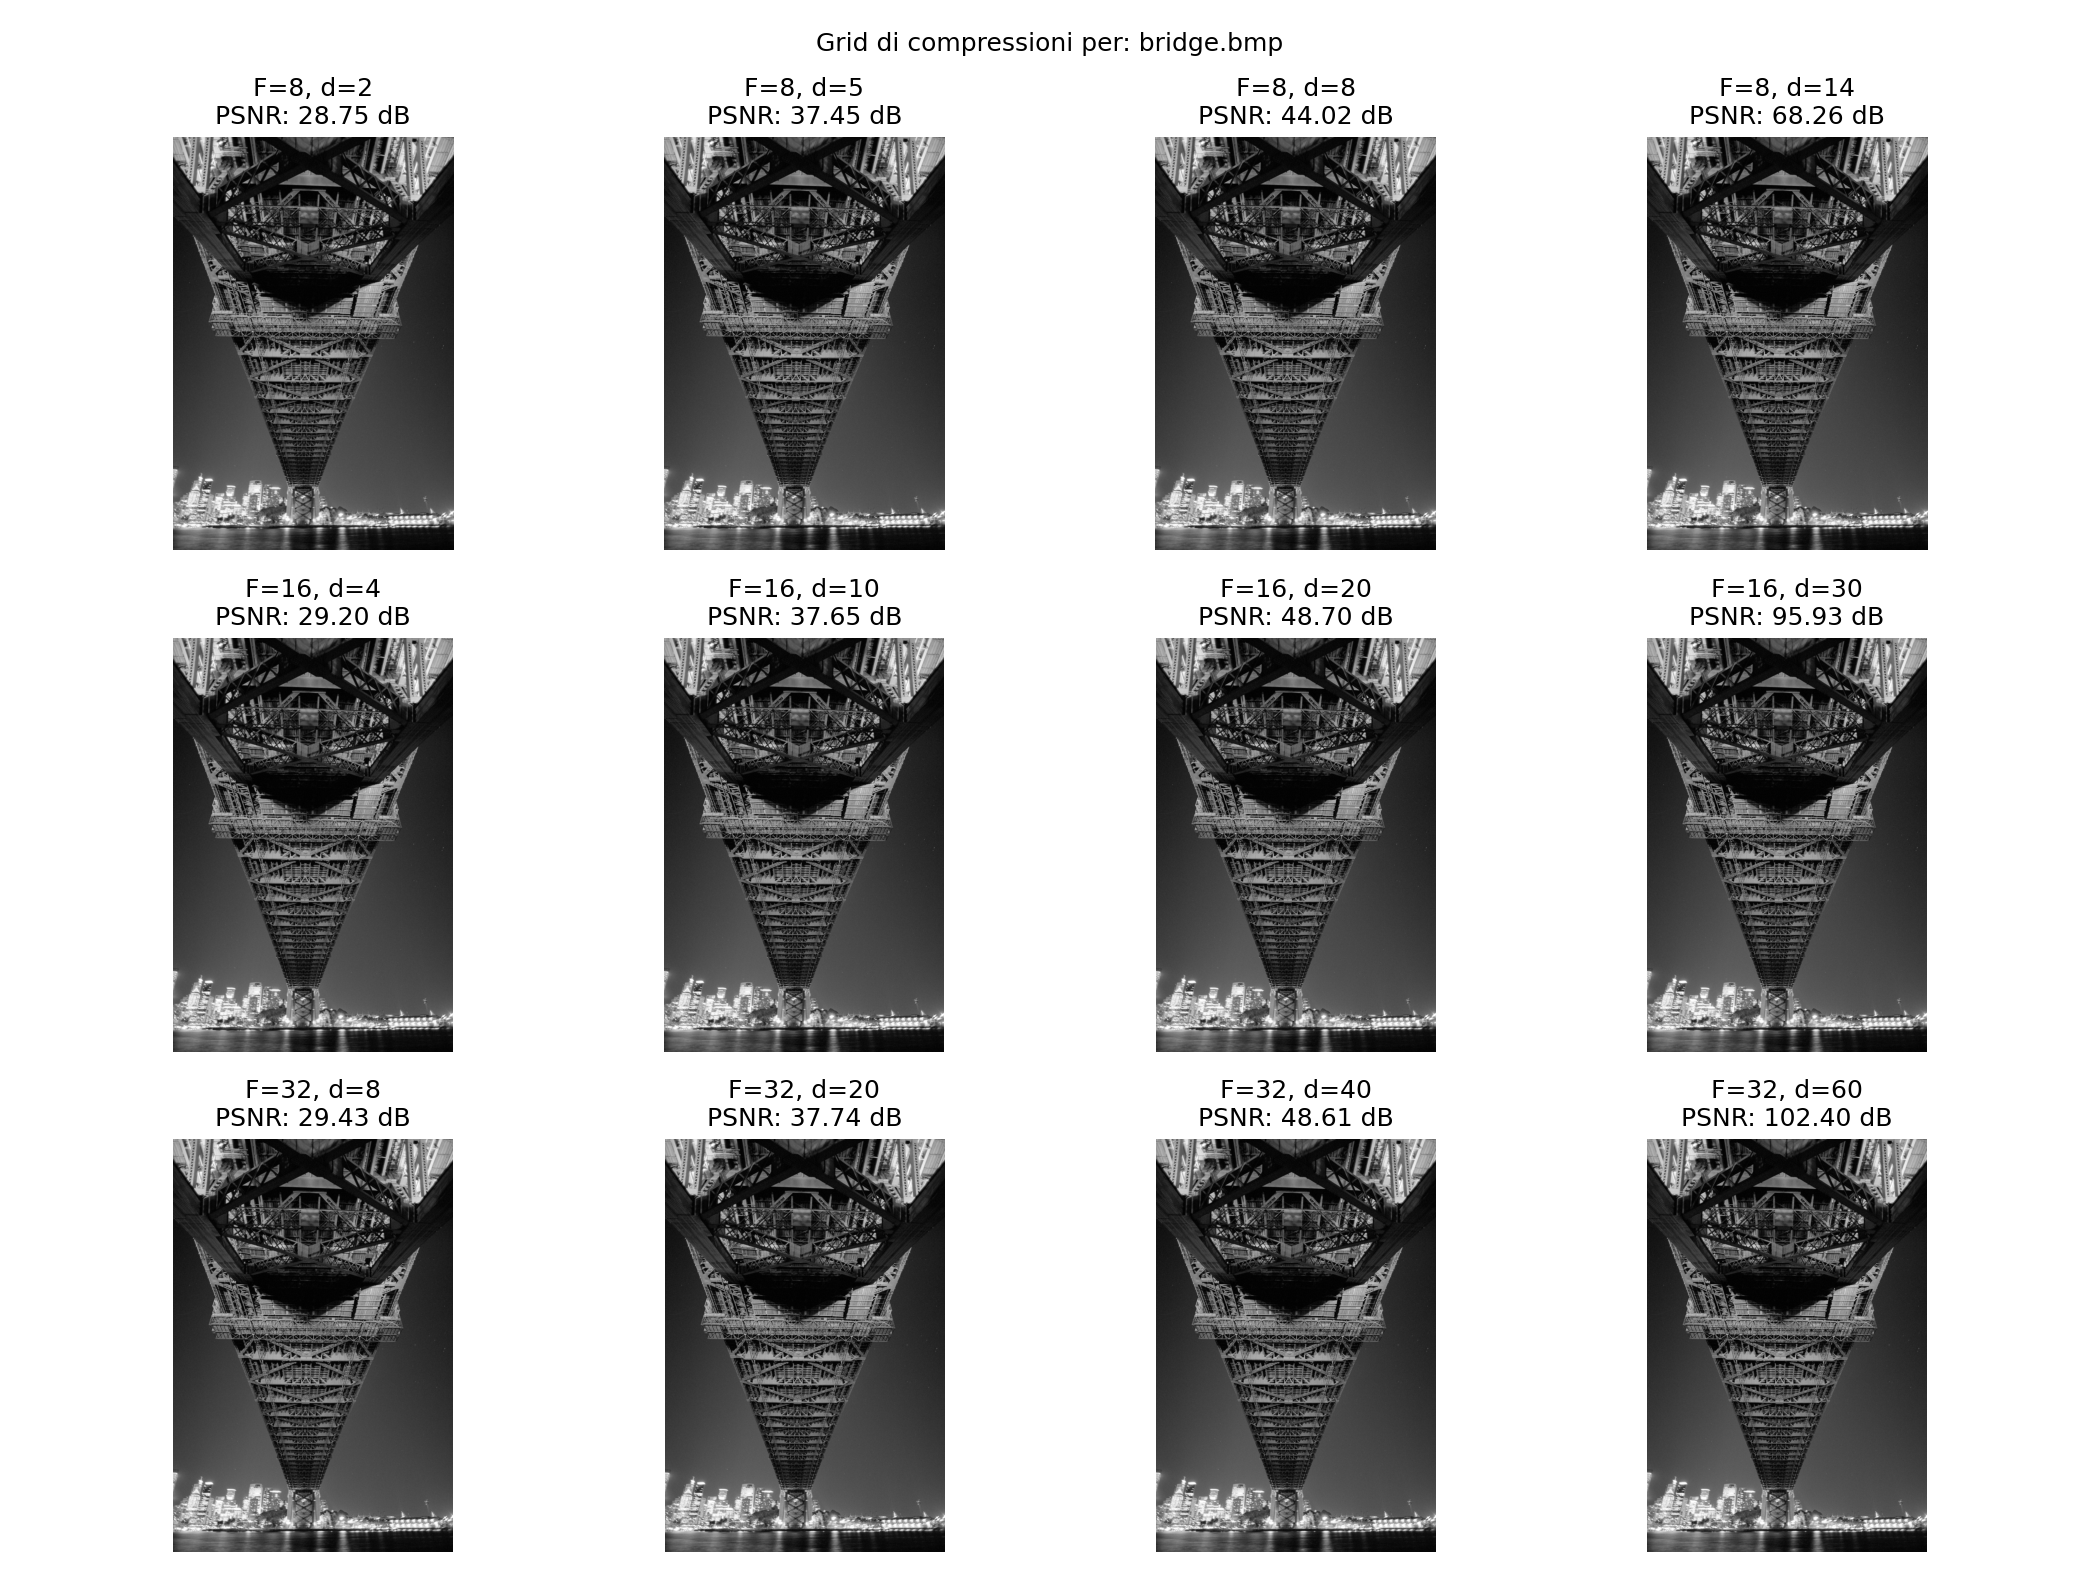
\includegraphics[width=\textwidth]{figures/bridge_grid.png}
\caption{\texttt{bridge} -- griglia}
\end{subfigure}
\begin{subfigure}{0.49\textwidth}\centering
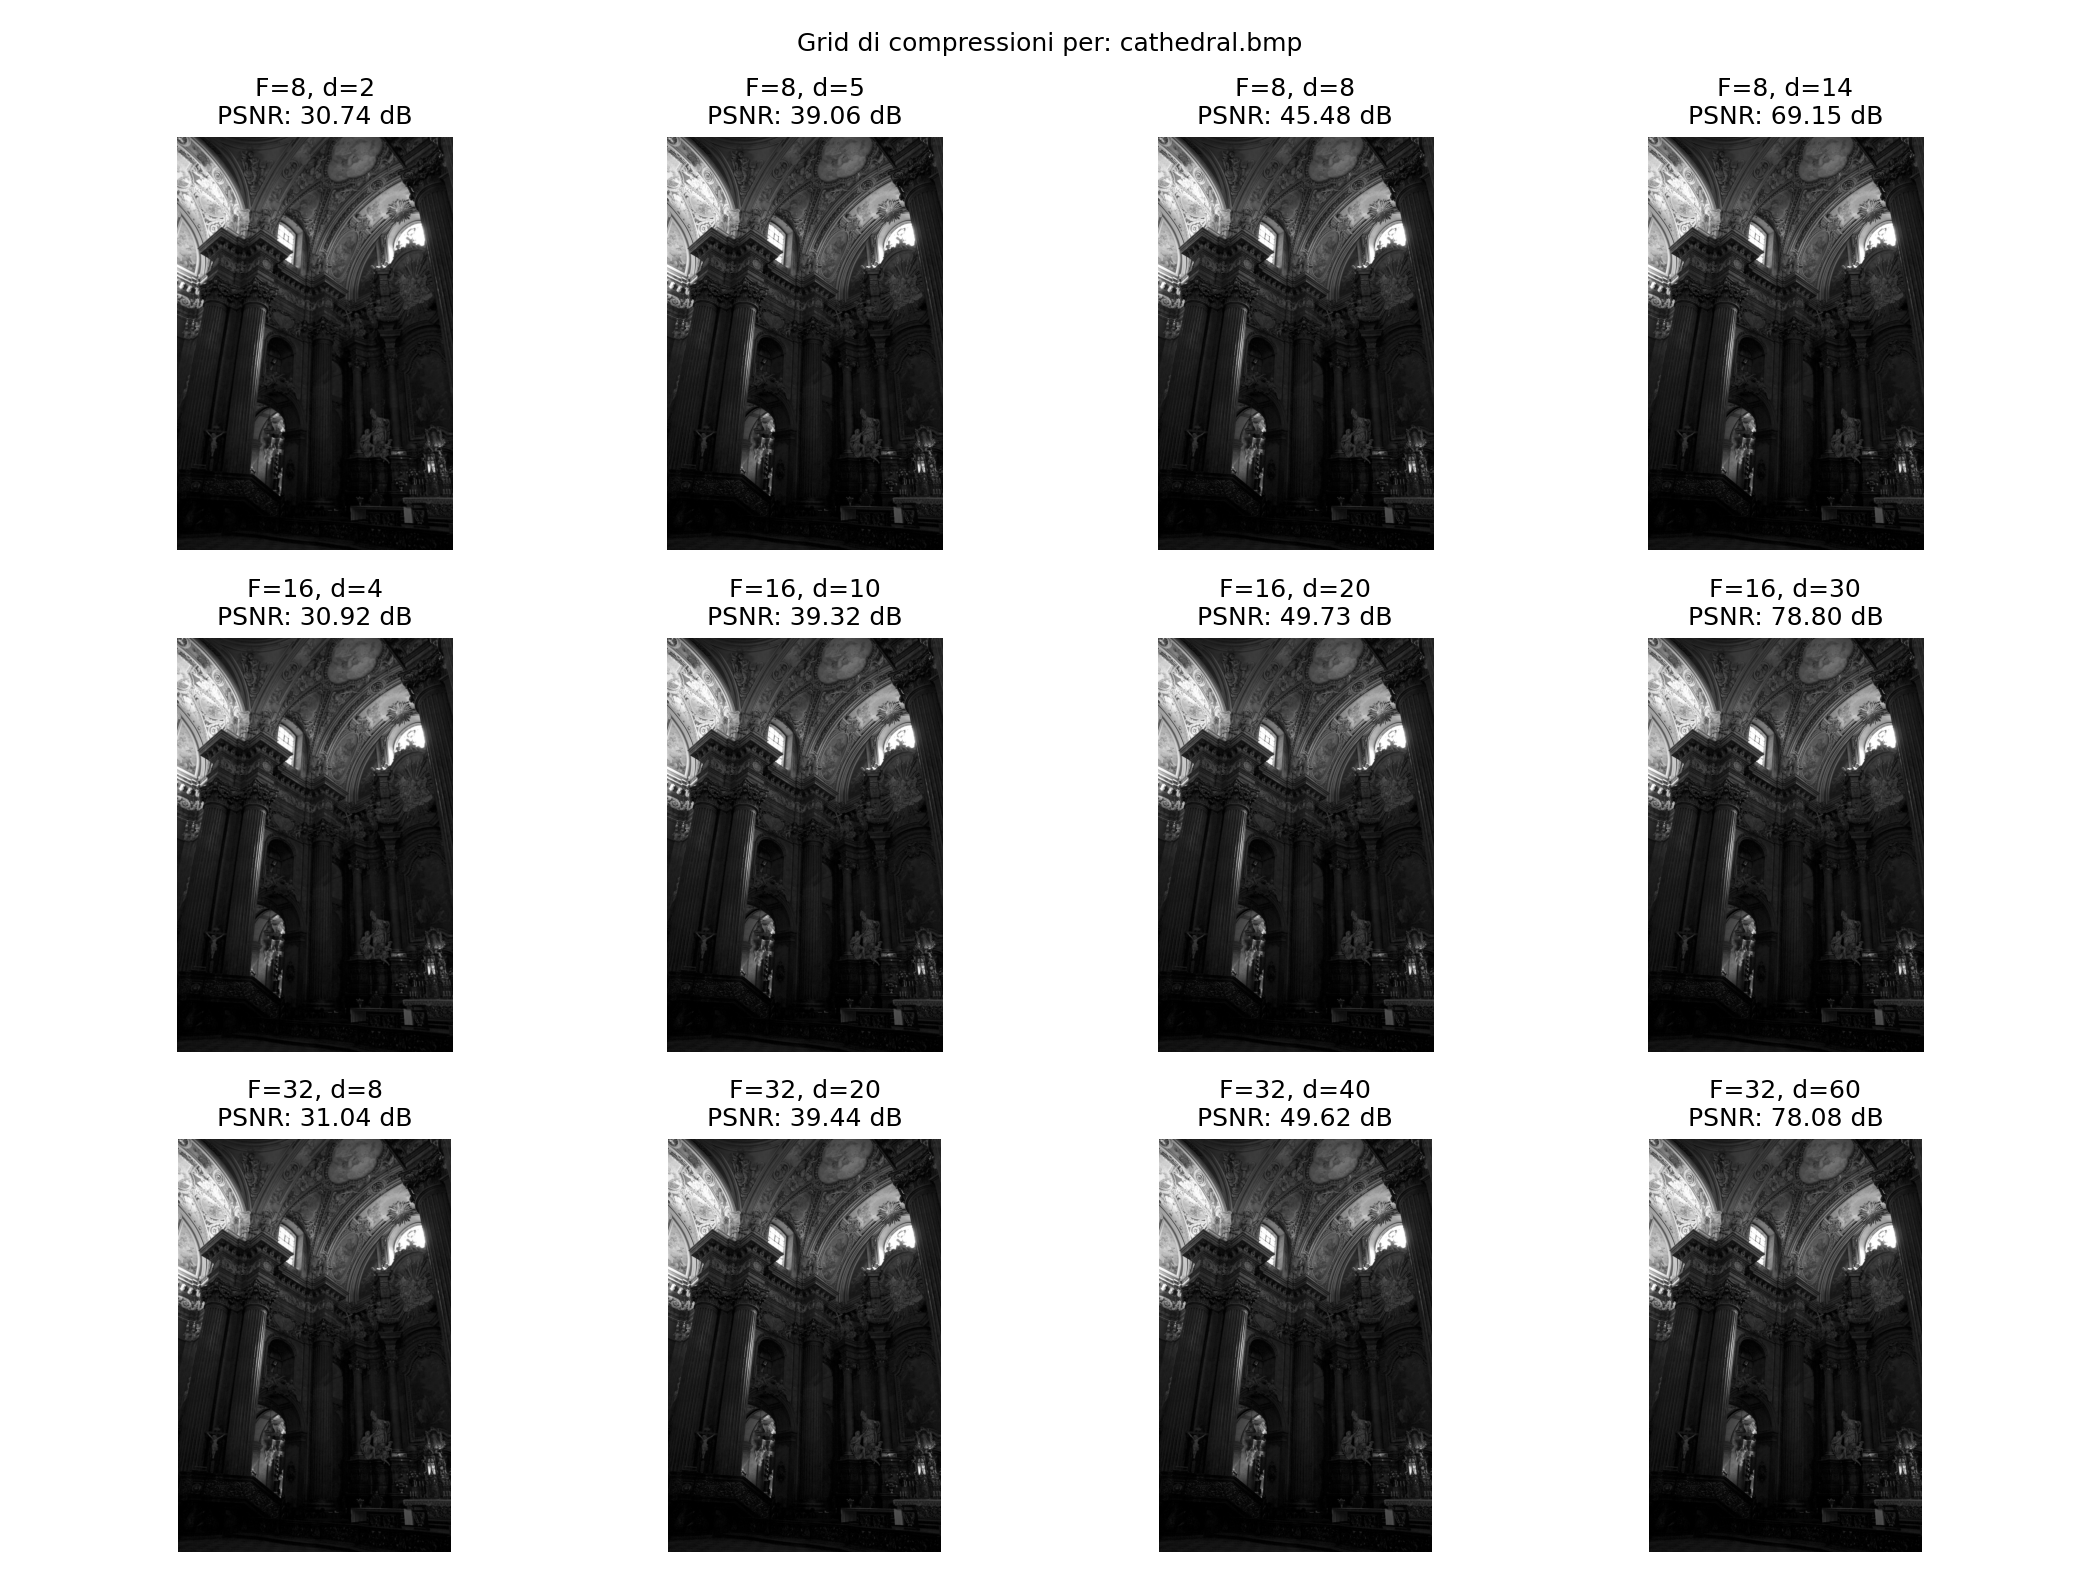
\includegraphics[width=\textwidth]{figures/cathedral_grid.png}
\caption{\texttt{cathedral} -- griglia}
\end{subfigure}
\caption{Griglie di compressione su due fotografie reali: $F=8,16,32$ a $d$
crescenti. Le foto naturali tollerano un taglio aggressivo molto meglio delle
scacchiere.}
\label{fig:bridge_cath}
\end{figure}

\begin{figure}[H]
\centering
\begin{subfigure}{0.49\textwidth}\centering
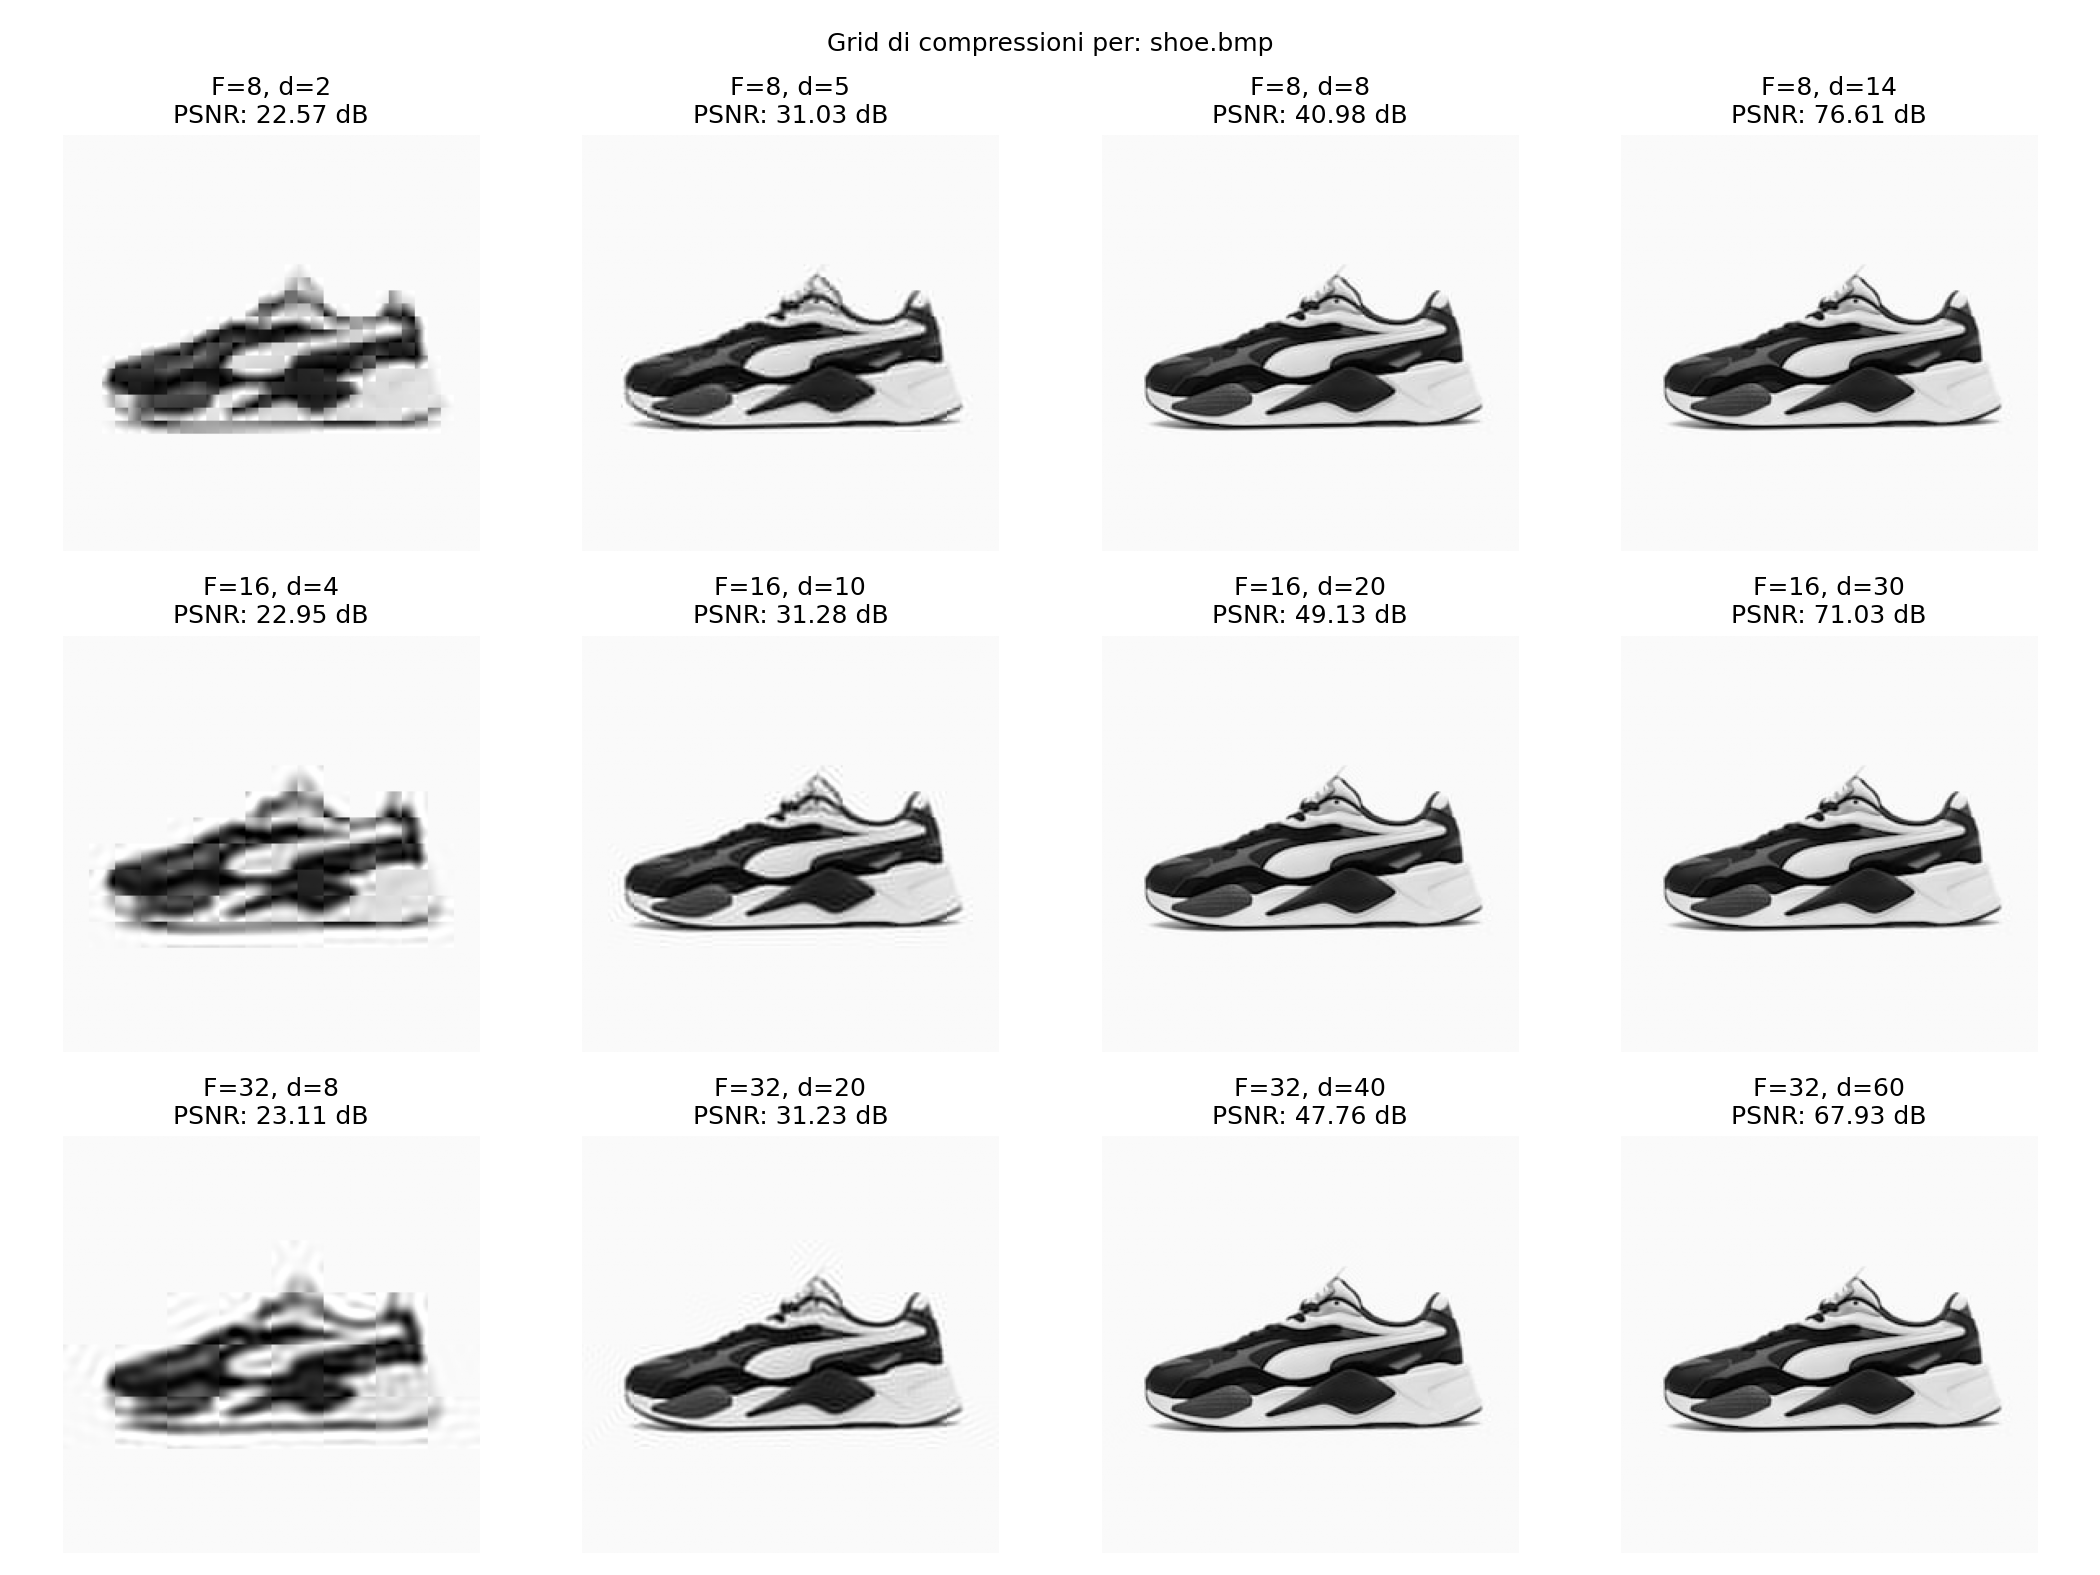
\includegraphics[width=\textwidth]{figures/shoe_grid.png}
\caption{\texttt{shoe}}
\end{subfigure}
\begin{subfigure}{0.49\textwidth}\centering
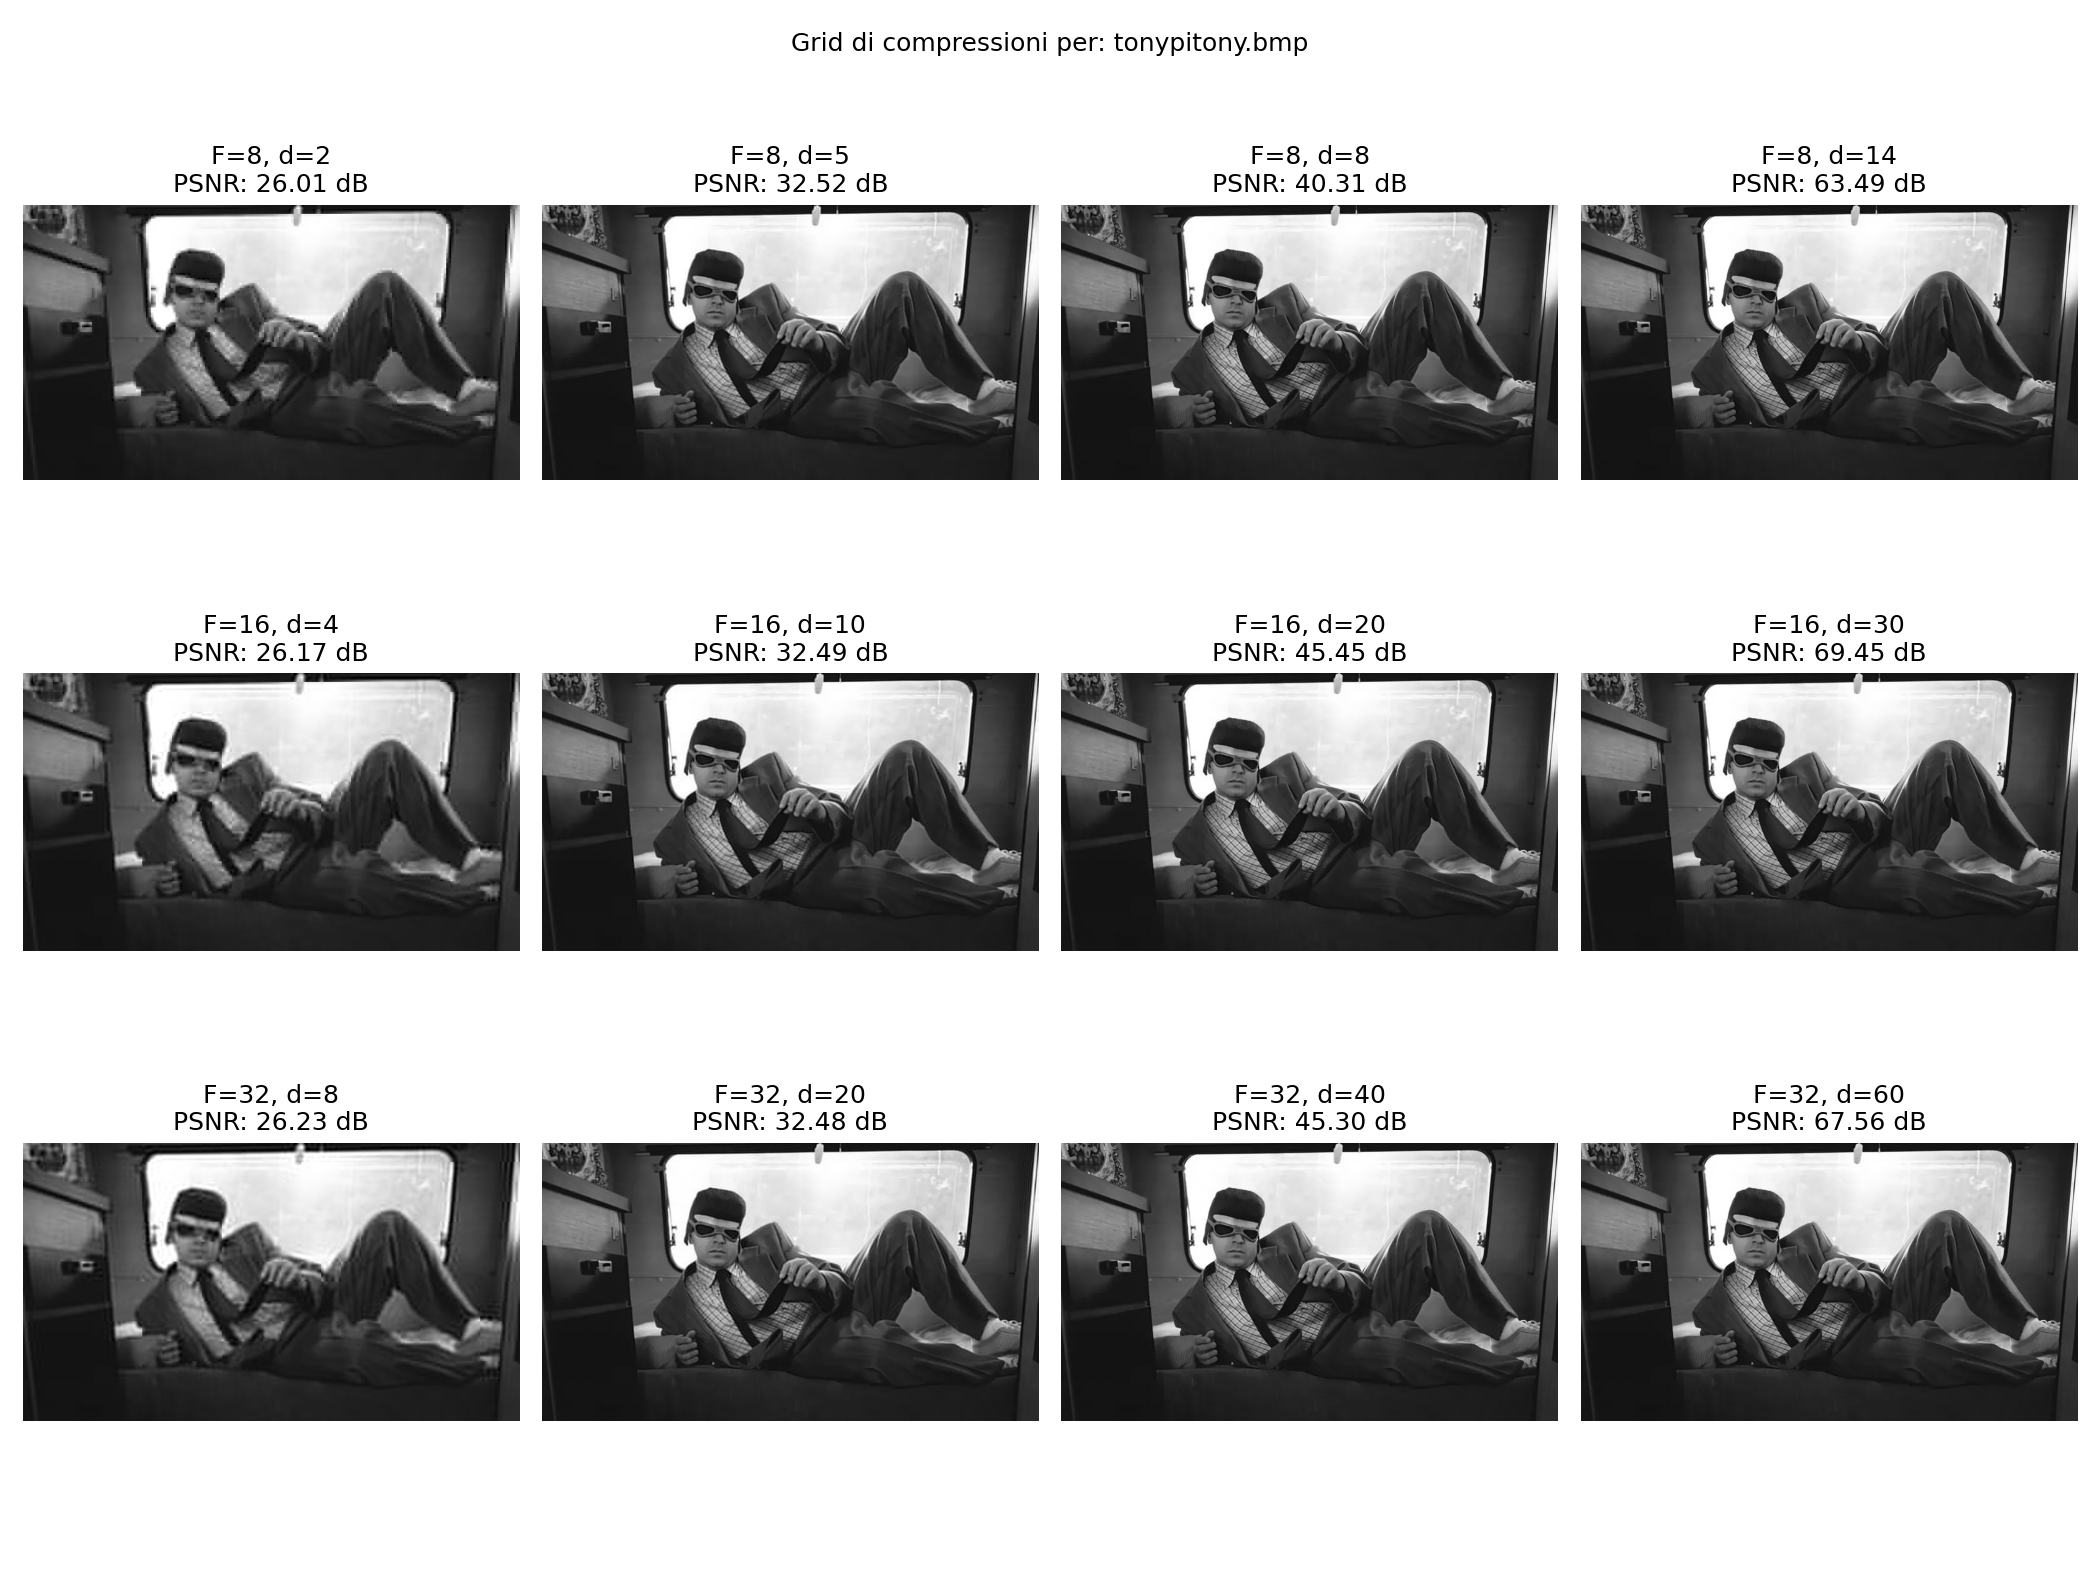
\includegraphics[width=\textwidth]{figures/tonypitony_grid.png}
\caption{\texttt{tonypitony}}
\end{subfigure}
\caption{Griglie di compressione su \texttt{shoe} e \texttt{tonypitony}.}
\label{fig:shoe_tony}
\end{figure}

\begin{figure}[H]
\centering
\begin{subfigure}{0.49\textwidth}\centering
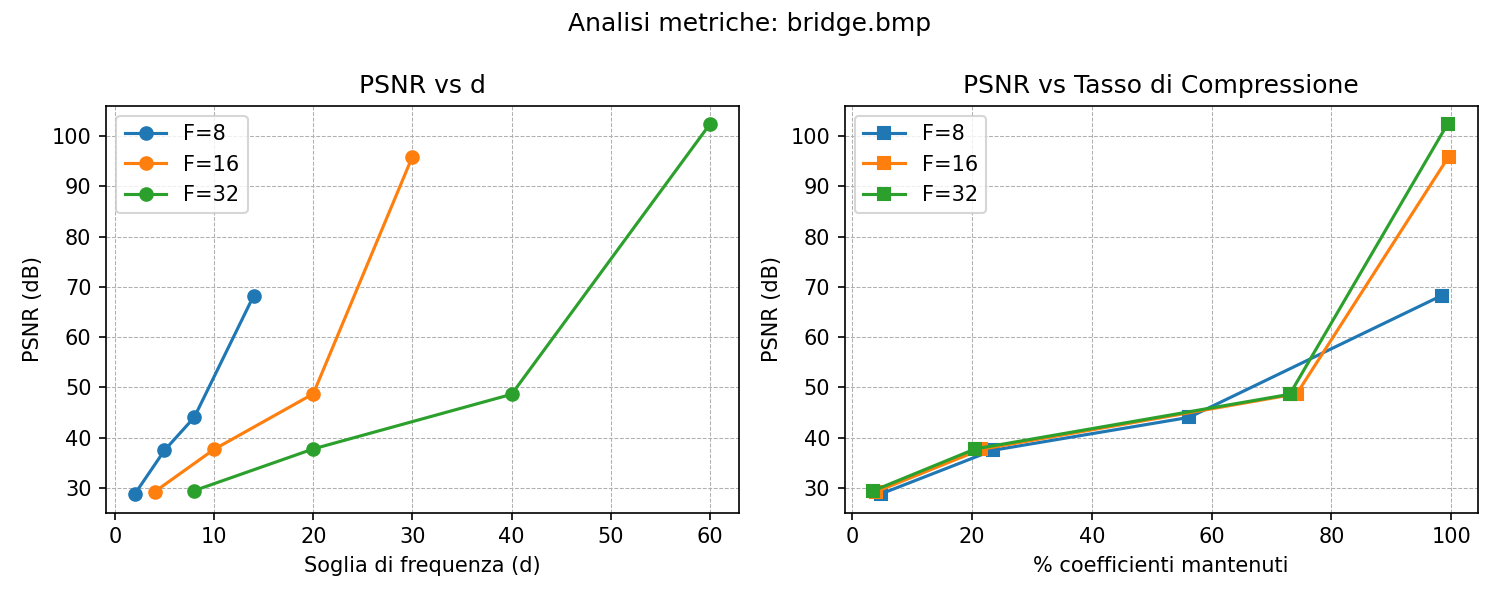
\includegraphics[width=\textwidth]{figures/bridge_metrics.png}
\caption{\texttt{bridge}}
\end{subfigure}
\begin{subfigure}{0.49\textwidth}\centering
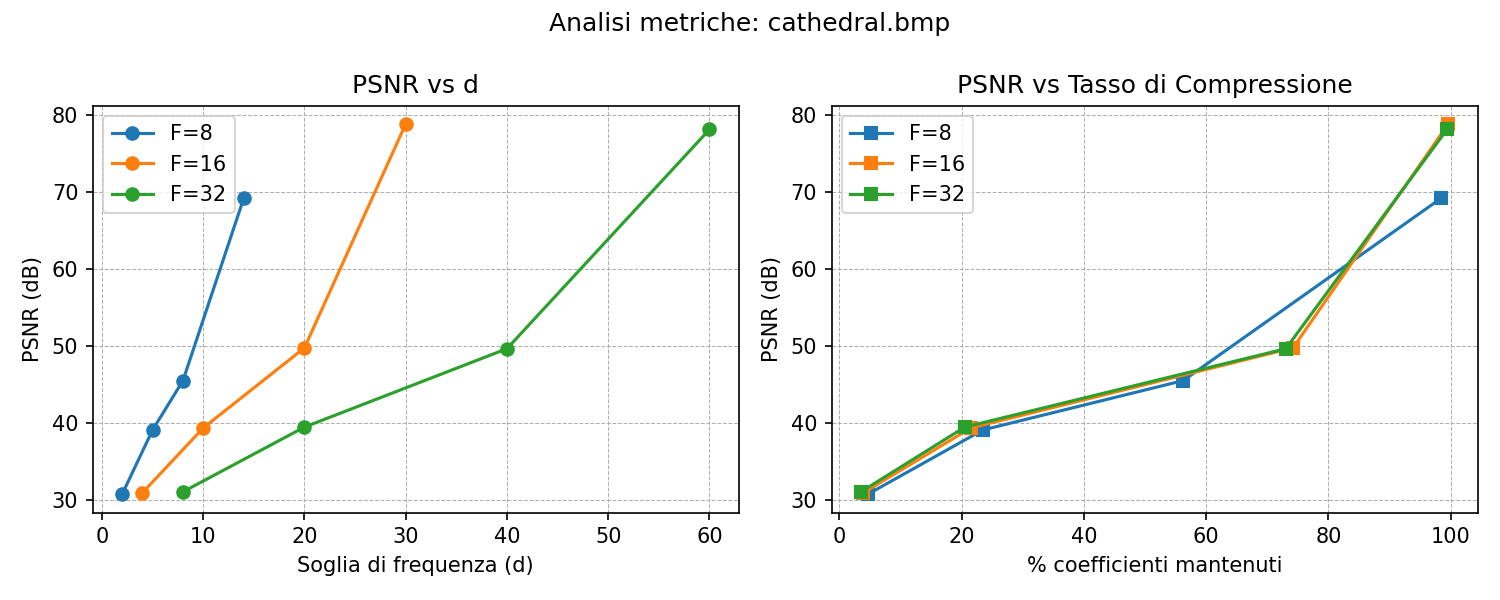
\includegraphics[width=\textwidth]{figures/cathedral_metrics.png}
\caption{\texttt{cathedral}}
\end{subfigure}
\caption{Metriche PSNR vs $d$ e vs \% coefficienti su \texttt{bridge} e
\texttt{cathedral}, per $F=8,16,32$.}
\label{fig:tonypitony}
\end{figure}

\subsection{Tabella dati completa}\label{sec:dati}

La Tabella~\ref{tab:dati} riporta l'elenco completo dei risultati sperimentali:
per ogni immagine e ogni coppia $(F,d)$, i valori di MSE, PSNR e percentuale di
coefficienti mantenuti. I valori di PSNR $\infty$ corrispondono a MSE $=0$
(ricostruzione esatta).

\begin{longtable}{llrrrr}
\caption{Dati sperimentali completi: MSE, PSNR [dB] e \% coefficienti mantenuti
per ogni immagine e ogni coppia $(F,d)$.}\label{tab:dati}\\
\toprule
Immagine & $F$ & $d$ & MSE & PSNR [dB] & coeff.\ tenuti \% \\
\midrule
\endfirsthead
\toprule
Immagine & $F$ & $d$ & MSE & PSNR [dB] & coeff.\ tenuti \% \\
\midrule
\endhead
\midrule
\multicolumn{6}{r}{\textit{continua nella pagina successiva}} \\
\endfoot
\bottomrule
\endlastfoot
deer & 8 & 2 & 72.03 & 29.56 & 4.69 \\
deer & 8 & 5 & 16.97 & 35.84 & 23.44 \\
deer & 8 & 8 & 4.11 & 41.99 & 56.25 \\
deer & 8 & 14 & 0.0160 & 66.09 & 98.44 \\
deer & 16 & 4 & 70.74 & 29.63 & 3.91 \\
deer & 16 & 10 & 16.90 & 35.85 & 21.48 \\
deer & 16 & 20 & 1.29 & 47.02 & 74.22 \\
deer & 16 & 30 & 0.00213 & 74.85 & 99.61 \\
deer & 32 & 8 & 71.53 & 29.59 & 3.52 \\
deer & 32 & 20 & 17.28 & 35.76 & 20.51 \\
deer & 32 & 40 & 1.35 & 46.83 & 73.05 \\
deer & 32 & 60 & 0.00241 & 74.31 & 99.41 \\
bridge & 8 & 2 & 86.79 & 28.75 & 4.69 \\
bridge & 8 & 5 & 11.69 & 37.45 & 23.44 \\
bridge & 8 & 8 & 2.58 & 44.02 & 56.25 \\
bridge & 8 & 14 & 0.0097 & 68.26 & 98.44 \\
bridge & 16 & 4 & 78.21 & 29.20 & 3.91 \\
bridge & 16 & 10 & 11.18 & 37.65 & 21.48 \\
bridge & 16 & 20 & 0.876 & 48.70 & 74.22 \\
bridge & 16 & 30 & 1.66e-05 & 95.93 & 99.61 \\
bridge & 32 & 8 & 74.11 & 29.43 & 3.52 \\
bridge & 32 & 20 & 10.95 & 37.74 & 20.51 \\
bridge & 32 & 40 & 0.896 & 48.61 & 73.05 \\
bridge & 32 & 60 & 3.74e-06 & 102.40 & 99.41 \\
cathedral & 8 & 2 & 54.78 & 30.74 & 4.69 \\
cathedral & 8 & 5 & 8.07 & 39.06 & 23.44 \\
cathedral & 8 & 8 & 1.84 & 45.48 & 56.25 \\
cathedral & 8 & 14 & 0.0079 & 69.15 & 98.44 \\
cathedral & 16 & 4 & 52.64 & 30.92 & 3.91 \\
cathedral & 16 & 10 & 7.60 & 39.32 & 21.48 \\
cathedral & 16 & 20 & 0.692 & 49.73 & 74.22 \\
cathedral & 16 & 30 & 0.000858 & 78.80 & 99.61 \\
cathedral & 32 & 8 & 51.22 & 31.04 & 3.52 \\
cathedral & 32 & 20 & 7.39 & 39.44 & 20.51 \\
cathedral & 32 & 40 & 0.710 & 49.62 & 73.05 \\
cathedral & 32 & 60 & 0.00101 & 78.08 & 99.41 \\
shoe & 8 & 2 & 359.88 & 22.57 & 4.69 \\
shoe & 8 & 5 & 51.30 & 31.03 & 23.44 \\
shoe & 8 & 8 & 5.19 & 40.98 & 56.25 \\
shoe & 8 & 14 & 0.00142 & 76.61 & 98.44 \\
shoe & 16 & 4 & 329.64 & 22.95 & 3.91 \\
shoe & 16 & 10 & 48.40 & 31.28 & 21.48 \\
shoe & 16 & 20 & 0.795 & 49.13 & 74.22 \\
shoe & 16 & 30 & 0.00513 & 71.03 & 99.61 \\
shoe & 32 & 8 & 317.63 & 23.11 & 3.52 \\
shoe & 32 & 20 & 48.95 & 31.23 & 20.51 \\
shoe & 32 & 40 & 1.089 & 47.76 & 73.05 \\
shoe & 32 & 60 & 0.01048 & 67.93 & 99.41 \\
tonypitony & 8 & 2 & 162.81 & 26.01 & 4.69 \\
tonypitony & 8 & 5 & 36.37 & 32.52 & 23.44 \\
tonypitony & 8 & 8 & 6.05 & 40.31 & 56.25 \\
tonypitony & 8 & 14 & 0.0291 & 63.49 & 98.44 \\
tonypitony & 16 & 4 & 157.18 & 26.17 & 3.91 \\
tonypitony & 16 & 10 & 36.69 & 32.49 & 21.48 \\
tonypitony & 16 & 20 & 1.85 & 45.45 & 74.22 \\
tonypitony & 16 & 30 & 0.00737 & 69.45 & 99.61 \\
tonypitony & 32 & 8 & 154.74 & 26.23 & 3.52 \\
tonypitony & 32 & 20 & 36.76 & 32.48 & 20.51 \\
tonypitony & 32 & 40 & 1.92 & 45.30 & 73.05 \\
tonypitony & 32 & 60 & 0.0114 & 67.56 & 99.41 \\
gradient & 8 & 2 & 0.238 & 54.37 & 4.69 \\
gradient & 8 & 5 & 0.177 & 55.64 & 23.44 \\
gradient & 8 & 8 & 0.0708 & 59.63 & 56.25 \\
gradient & 8 & 14 & 0 & $\infty$ & 98.44 \\
gradient & 16 & 4 & 0.239 & 54.35 & 3.91 \\
gradient & 16 & 10 & 0.182 & 55.53 & 21.48 \\
gradient & 16 & 20 & 0.0201 & 65.10 & 74.22 \\
gradient & 16 & 30 & 0 & $\infty$ & 99.61 \\
gradient & 32 & 8 & 0.239 & 54.35 & 3.52 \\
gradient & 32 & 20 & 0.186 & 55.44 & 20.51 \\
gradient & 32 & 40 & 0.0207 & 64.96 & 73.05 \\
gradient & 32 & 60 & 0 & $\infty$ & 99.41 \\
prova & 8 & 2 & 1180.24 & 17.41 & 4.69 \\
prova & 8 & 5 & 381.04 & 22.32 & 23.44 \\
prova & 8 & 8 & 129.95 & 26.99 & 56.25 \\
prova & 8 & 14 & 3.05 & 43.28 & 98.44 \\
prova & 16 & 4 & 1048.99 & 17.92 & 3.91 \\
prova & 16 & 10 & 366.18 & 22.49 & 21.48 \\
prova & 16 & 20 & 56.38 & 30.62 & 74.22 \\
prova & 16 & 30 & 0.929 & 48.45 & 99.61 \\
prova & 32 & 8 & 999.43 & 18.13 & 3.52 \\
prova & 32 & 20 & 357.67 & 22.60 & 20.51 \\
prova & 32 & 40 & 54.77 & 30.75 & 73.05 \\
prova & 32 & 60 & 1.17 & 47.43 & 99.41 \\
320x320 & 8 & 2 & 6667.81 & 9.89 & 4.69 \\
320x320 & 8 & 5 & 1357.91 & 16.80 & 23.44 \\
320x320 & 8 & 8 & 219.40 & 24.72 & 56.25 \\
320x320 & 8 & 14 & 1.48 & 46.44 & 98.44 \\
320x320 & 16 & 4 & 6532.25 & 9.98 & 3.91 \\
320x320 & 16 & 10 & 1569.60 & 16.17 & 21.48 \\
320x320 & 16 & 20 & 51.95 & 30.97 & 74.22 \\
320x320 & 16 & 30 & 0.199 & 55.15 & 99.61 \\
320x320 & 32 & 8 & 5562.54 & 10.68 & 3.52 \\
320x320 & 32 & 20 & 1599.81 & 16.09 & 20.51 \\
320x320 & 32 & 40 & 50.60 & 31.09 & 73.05 \\
320x320 & 32 & 60 & 0.0263 & 63.94 & 99.41 \\
\end{longtable}

\subsection{Commenti finali}\label{sec:commenti}

Gli esperimenti illustrano i due fenomeni principali della compressione DCT a
blocchi:
\begin{enumerate}
  \item Su \emph{zone regolari} dell'immagine bastano pochissimi coefficienti
        per ricostruirla con buona qualità, perché i coefficienti di indice
        alto decadono rapidamente: è il meccanismo che rende efficace la
        compressione JPEG.
  \item In presenza di \emph{discontinuità} (bordi netti, contorni di oggetti)
        troncare le alte frequenze produce oscillazioni spurie (Gibbs)
        localizzate vicino al bordo. La suddivisione a macro-blocchi confina il
        problema all'interno di ciascun blocco, ma rende contemporaneamente
        visibile lo schema della partizione quando $d$ è troppo piccolo rispetto
        a $F$.
\end{enumerate}
Il valore $F=8$ usato nel JPEG è un ottimo compromesso: con blocchi più grandi
l'algoritmo \guillemotleft comprenderebbe\guillemotright{} meglio il contesto
generale, ma gli artefatti ricadrebbero su aree più ampie e il costo
computazionale crescerebbe (come $O(F^2\log F)$); con blocchi più piccoli
l'algoritmo sarebbe più veloce, ma meno efficace nel concentrare
l'informazione sulle basse frequenze.

\section{Conclusioni}\label{sec:conclusioni}

Si è implementata in Python una DCT2 ortonormale come richiesto dal progetto
(matrice $D$ esplicita, costo $O(N^3)$) e la si è confrontata sperimentalmente
con la versione \emph{fast} di \texttt{scipy.fft}, verificando che i tempi
seguano le complessità $N^3$ e $N^2\log N$. Si è quindi usata la versione fast
per realizzare un software di compressione di immagini in scala di grigio
secondo lo schema indicato dalla traccia, dotato di interfaccia grafica
\texttt{tkinter}. Gli esperimenti su immagini con bordi netti e fotografiche
hanno confermato le caratteristiche attese della compressione DCT: rapido
decadimento dei coefficienti per immagini lisce e comparsa di artefatti di
Gibbs in prossimità dei margini netti quando la soglia di taglio è troppo
aggressiva.

\appendix
\section{Codice sorgente}\label{app:codice}

Di seguito si riporta il codice sorgente completo dei moduli principali del
progetto. I file sono organizzati come descritto nella
Sezione~\ref{sec:struttura}.

\subsection{\texttt{dct\_utils.py}}
\lstinputlisting[language=Python]{code/dct_utils.py}

\subsection{\texttt{run\_assignment.py}}
\lstinputlisting[language=Python]{code/run_assignment.py}

\subsection{\texttt{gui.py}}
\lstinputlisting[language=Python]{code/gui.py}

\subsection{\texttt{test\_assignment.py}}
\lstinputlisting[language=Python]{code/test_assignment.py}

\end{document}
